\documentclass{article}
\usepackage{graphicx} % Required for inserting images
\usepackage[italian]{babel}
\usepackage[margin=3cm]{geometry}
\renewcommand{\familydefault}{\sfdefault}
\usepackage{float}
\usepackage{booktabs}
\usepackage{hyperref}
\usepackage{siunitx}

\title{Applicazione dell'algoritmo HITS a diverse tipologie di dati su modelli/sistemi e domande/topic}
\author{Gaia Simeoni}
\date{July 2025}

\begin{document}

\maketitle

\tableofcontents

\section{Applicazione HITS ai dati su modelli e domande}

\subsection{Hubness vs. Model effectiveness (MAP)}

\begin{figure}[H]
  \centering
  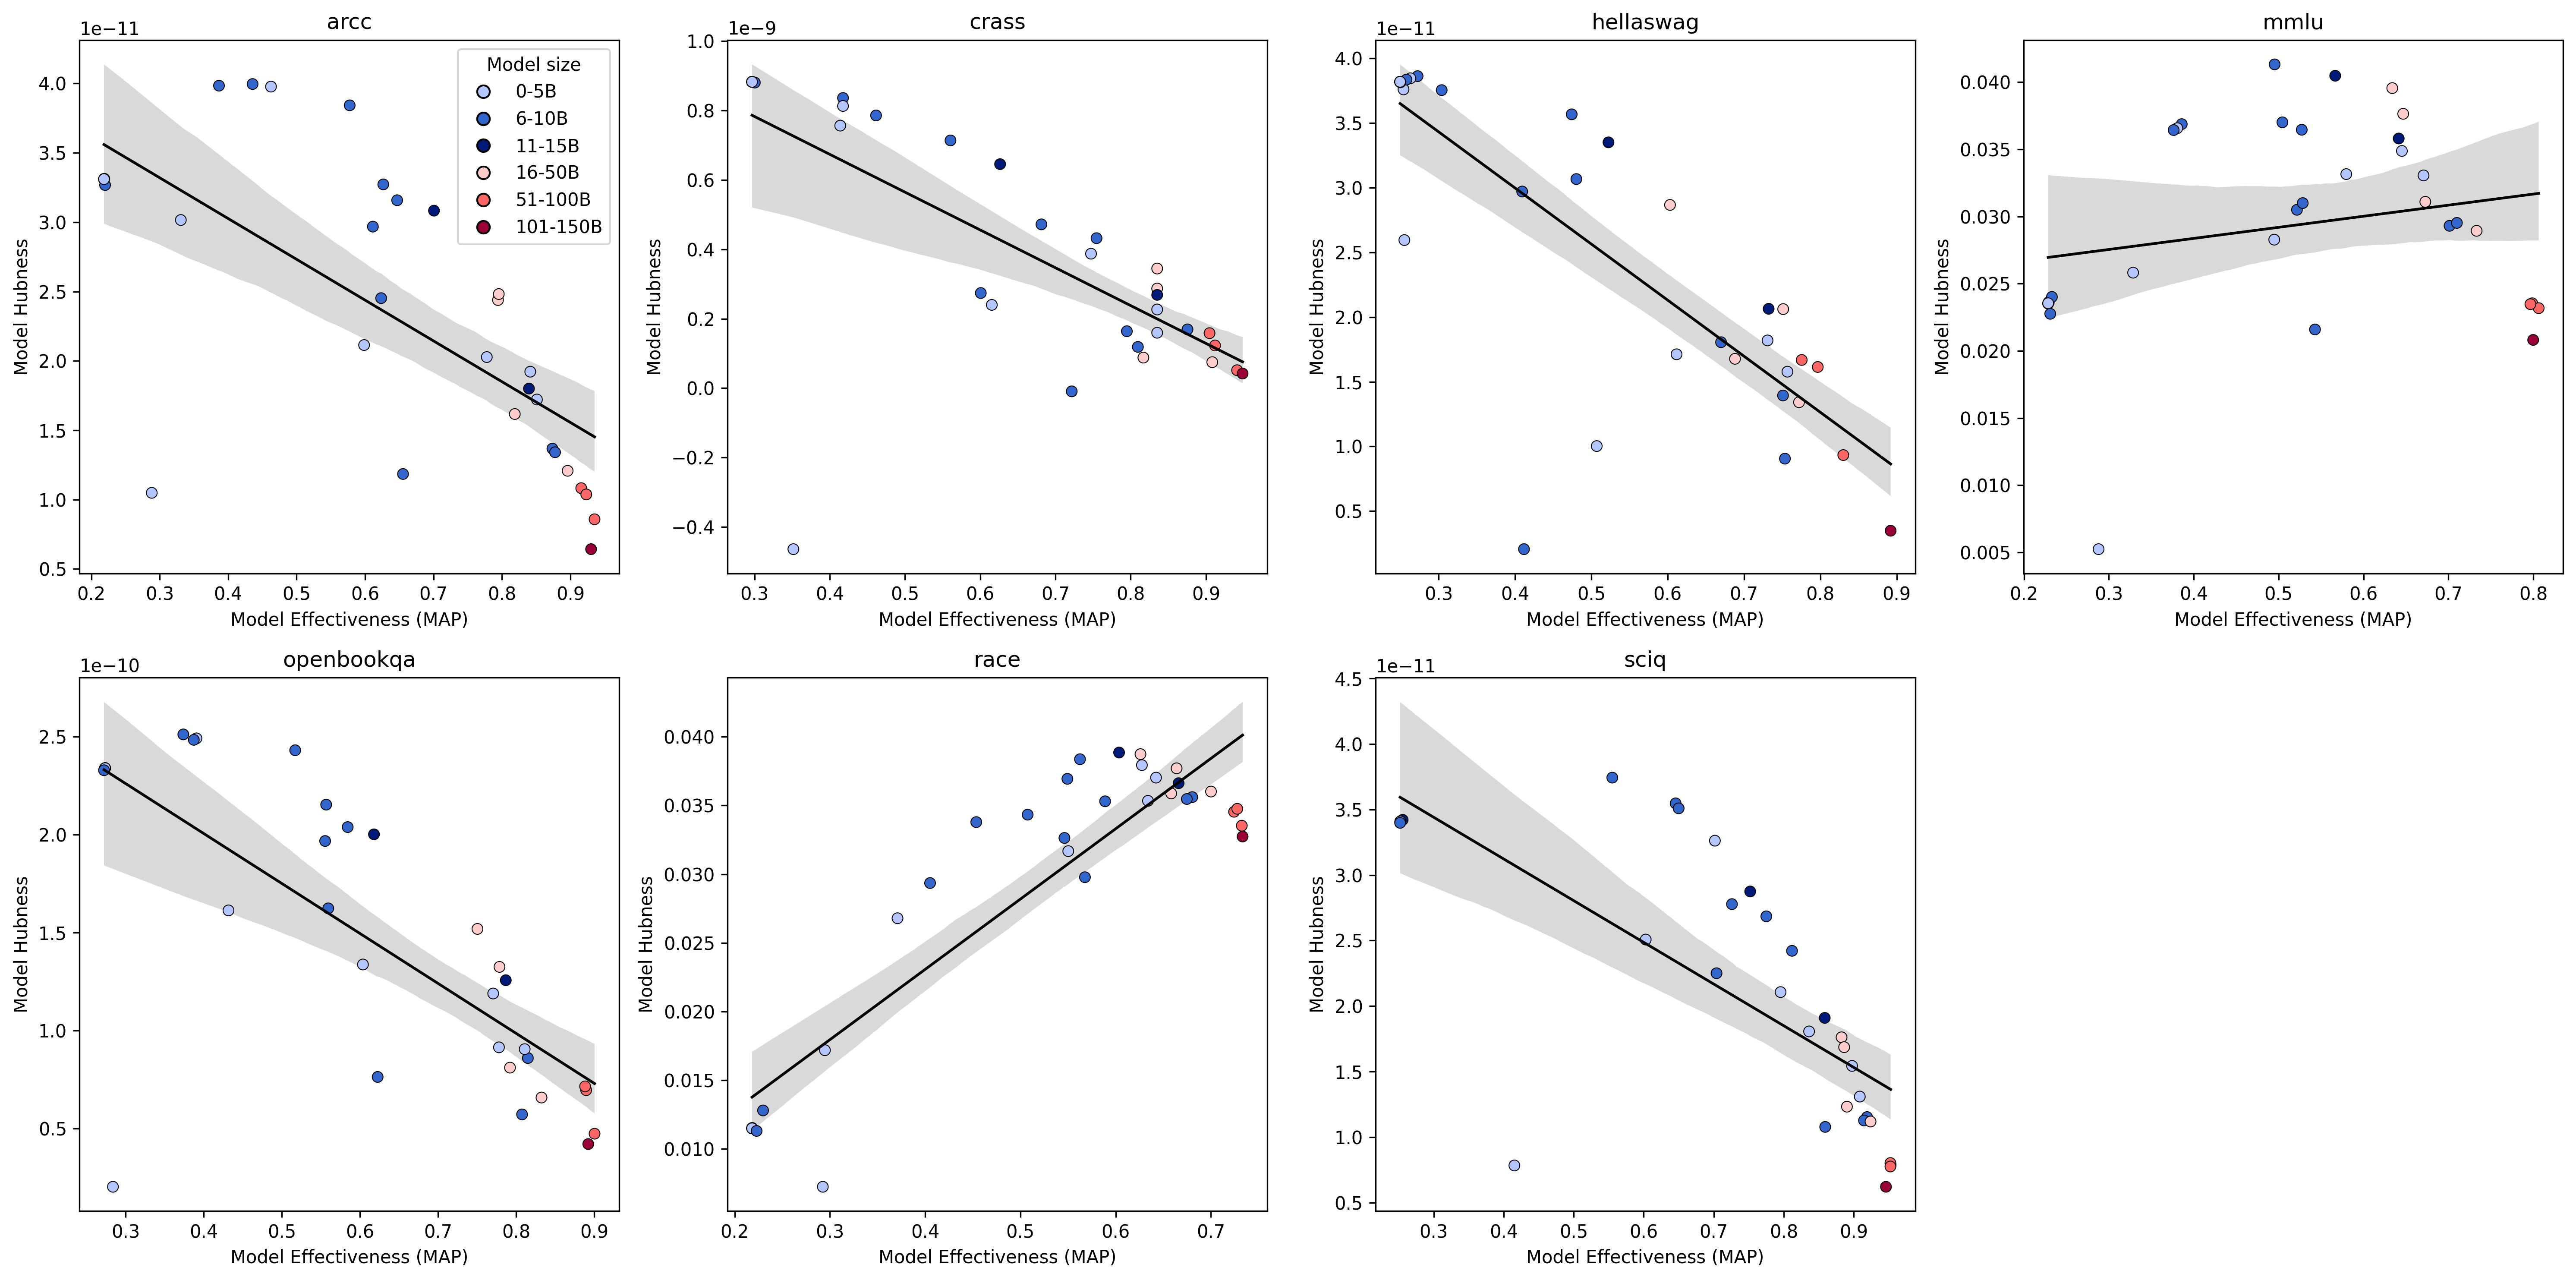
\includegraphics[width=0.9\linewidth]{images/plotsLLM/MAP_vs_Hubness_LLM_all_datasets.jpg}
  \caption{Relazione tra i valori di hubness dei modelli e l'efficacia dei modelli (misurata da MAP)}
  \label{fig:M_MAPvsHUB}
\end{figure}

Dai grafici in Figura \ref{fig:M_MAPvsHUB} è possibile notare che:

\begin{itemize}
  \item  Per crass, arcc, openbookqa, sciq, hellaswag: si osserva una correlazione
        prevalentemente negativa. Cioè, modelli più efficaci (MAP più alto) tendono ad
        avere un valore di hubness più bassa;
  \item Per race: correlazione positiva. Modelli più efficaci hanno hubness più alta;
  \item Per mmlu: correlazione debolmente positiva o quasi piatta.
\end{itemize}

Secondo l'algoritmo HITS, un buon hub è un nodo che punta a molte buone
autorità. Un "modello hub" è quindi un modello capace di rispondere
correttamente a molte "domande autorità", le quali sono generalmente domande
facili. Logicamente, se un modello con un MAP più alto (più efficace) è in
grado di risolvere domande più difficili, dovrebbe mostrare una hubness
inferiore, poiché la sua "hubness" è legata alla capacità di rispondere a
domande facili.

Il trend negativo osservato nei dataset crass, arcc, openbookqa, sciq e
hellaswag supporta questa ipotesi. Questo implica che i sistemi più efficaci
sono "meno bravi" a risolvere/riconoscere domande facili. Sebbene ciò possa
sembrare contro-intuitivo (ci si aspetterebbe che i modelli più efficaci
rispondano meglio anche alle domande facili), può essere spiegato in due modi:
i modelli più efficaci si concentrano sulla risoluzione di domande complesse,
riducendo la loro "hubness" sulle domande facili; oppure, i modelli meno
efficaci appaiono più "hub" proprio perché eccellono maggiormente nelle domande
facili, non essendo in grado di gestire quelle più difficili.

Per i dataset mmlu e race, la correlazione positiva o addirittura piatta è più
coerente perché sembrerebbe che modelli più efficaci non sono peggiori nel
riconoscere/rispondere a domande facili.

Si osserva quindi un trade-off tra specializzazione e generalizzazione delle
prestazioni: un modello può privilegiare la risoluzione di quesiti semplici
(domande authority) o puntare a mantenere buone performance anche su problemi
complessi. La hubness non è indice di eccellenza, ma riflette la tendenza a
concentrarsi su domande consensuali, che anche modelli meno performanti
risolvono correttamente. Valori elevati di hubness indicano quindi un’elevata
focalizzazione su quesiti facili. Tuttavia, per ottenere prestazioni di livello
superiore (alta MAP) è necessario superare questa specializzazione, dimostrando
capacità di risoluzione anche su problemi difficili e non consensuali.

\subsection{Authority vs Model effectiveness (MAP)}

\begin{figure}[H]
  \centering
  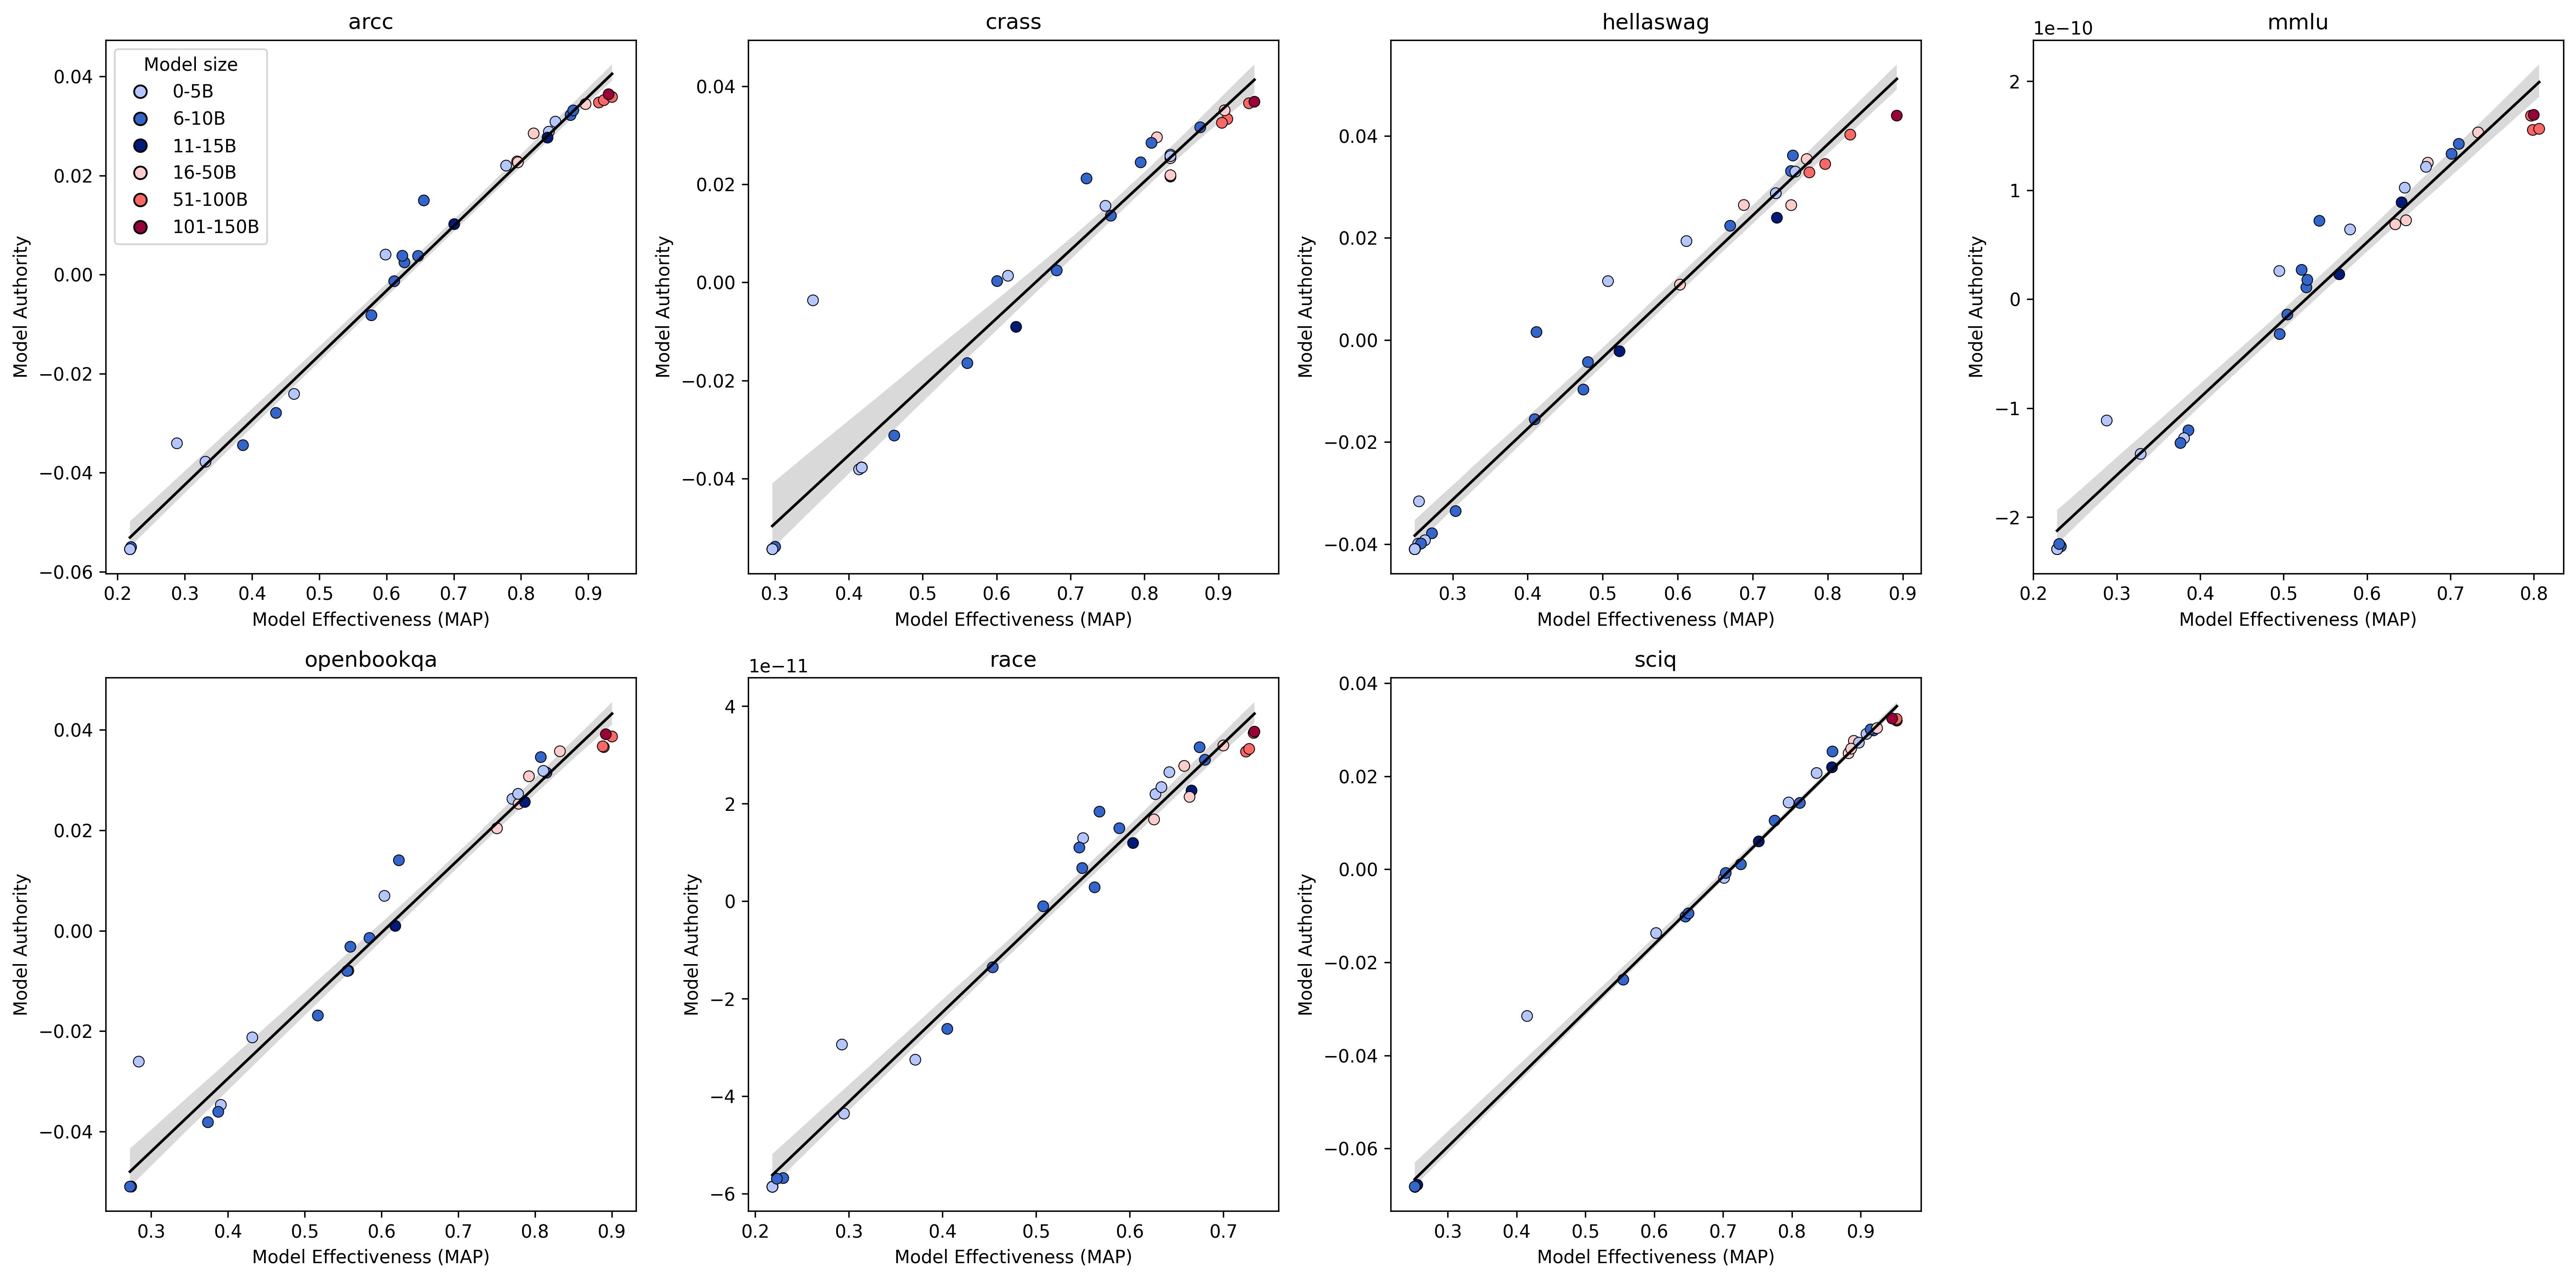
\includegraphics[width=0.9\linewidth]{images/plotsLLM/MAP_vs_Authority_LLM_all_datasets.jpg}
  \caption{Relazione tra i valori di authority dei modelli e l'efficacia dei modelli (misurata da MAP)}
  \label{fig:M_MAPvsAUTH}
\end{figure}

In generale dai grafici in Figura \ref{fig:M_MAPvsAUTH} si osserva una
correlazione positiva molto forte in tutti i dataset.

Secondo l'algoritmo HITS, un buon "authority" è un nodo puntato da molti buoni
"hub". Un "modello authority" è quindi un modello "riconosciuto" da molte
"domande hub", ossia domande capaci di evidenziare e discriminare le differenze
di efficacia tra i sistemi. Il trend positivo e l'elevata correlazione tra MAP
e authority in tutti i dataset suggeriscono che il punteggio di authority,
calcolato dall'algoritmo, è un buon indicatore dell'efficacia dei modelli. In
altre parole, i modelli con MAP più alto (più efficaci) tendono a essere
riconosciuti come "authority" da molte domande hub.

In conclusione il "prestigio" (authority) che HITS calcola e la "bravura" (MAP)
tendono a convergere: un’alta authority indica un modello riconosciuto come
performante soprattutto nella risoluzione delle domande più difficili.

\subsection{Hubness vs Question ease (AAP)}

\begin{figure}[H]
  \centering
  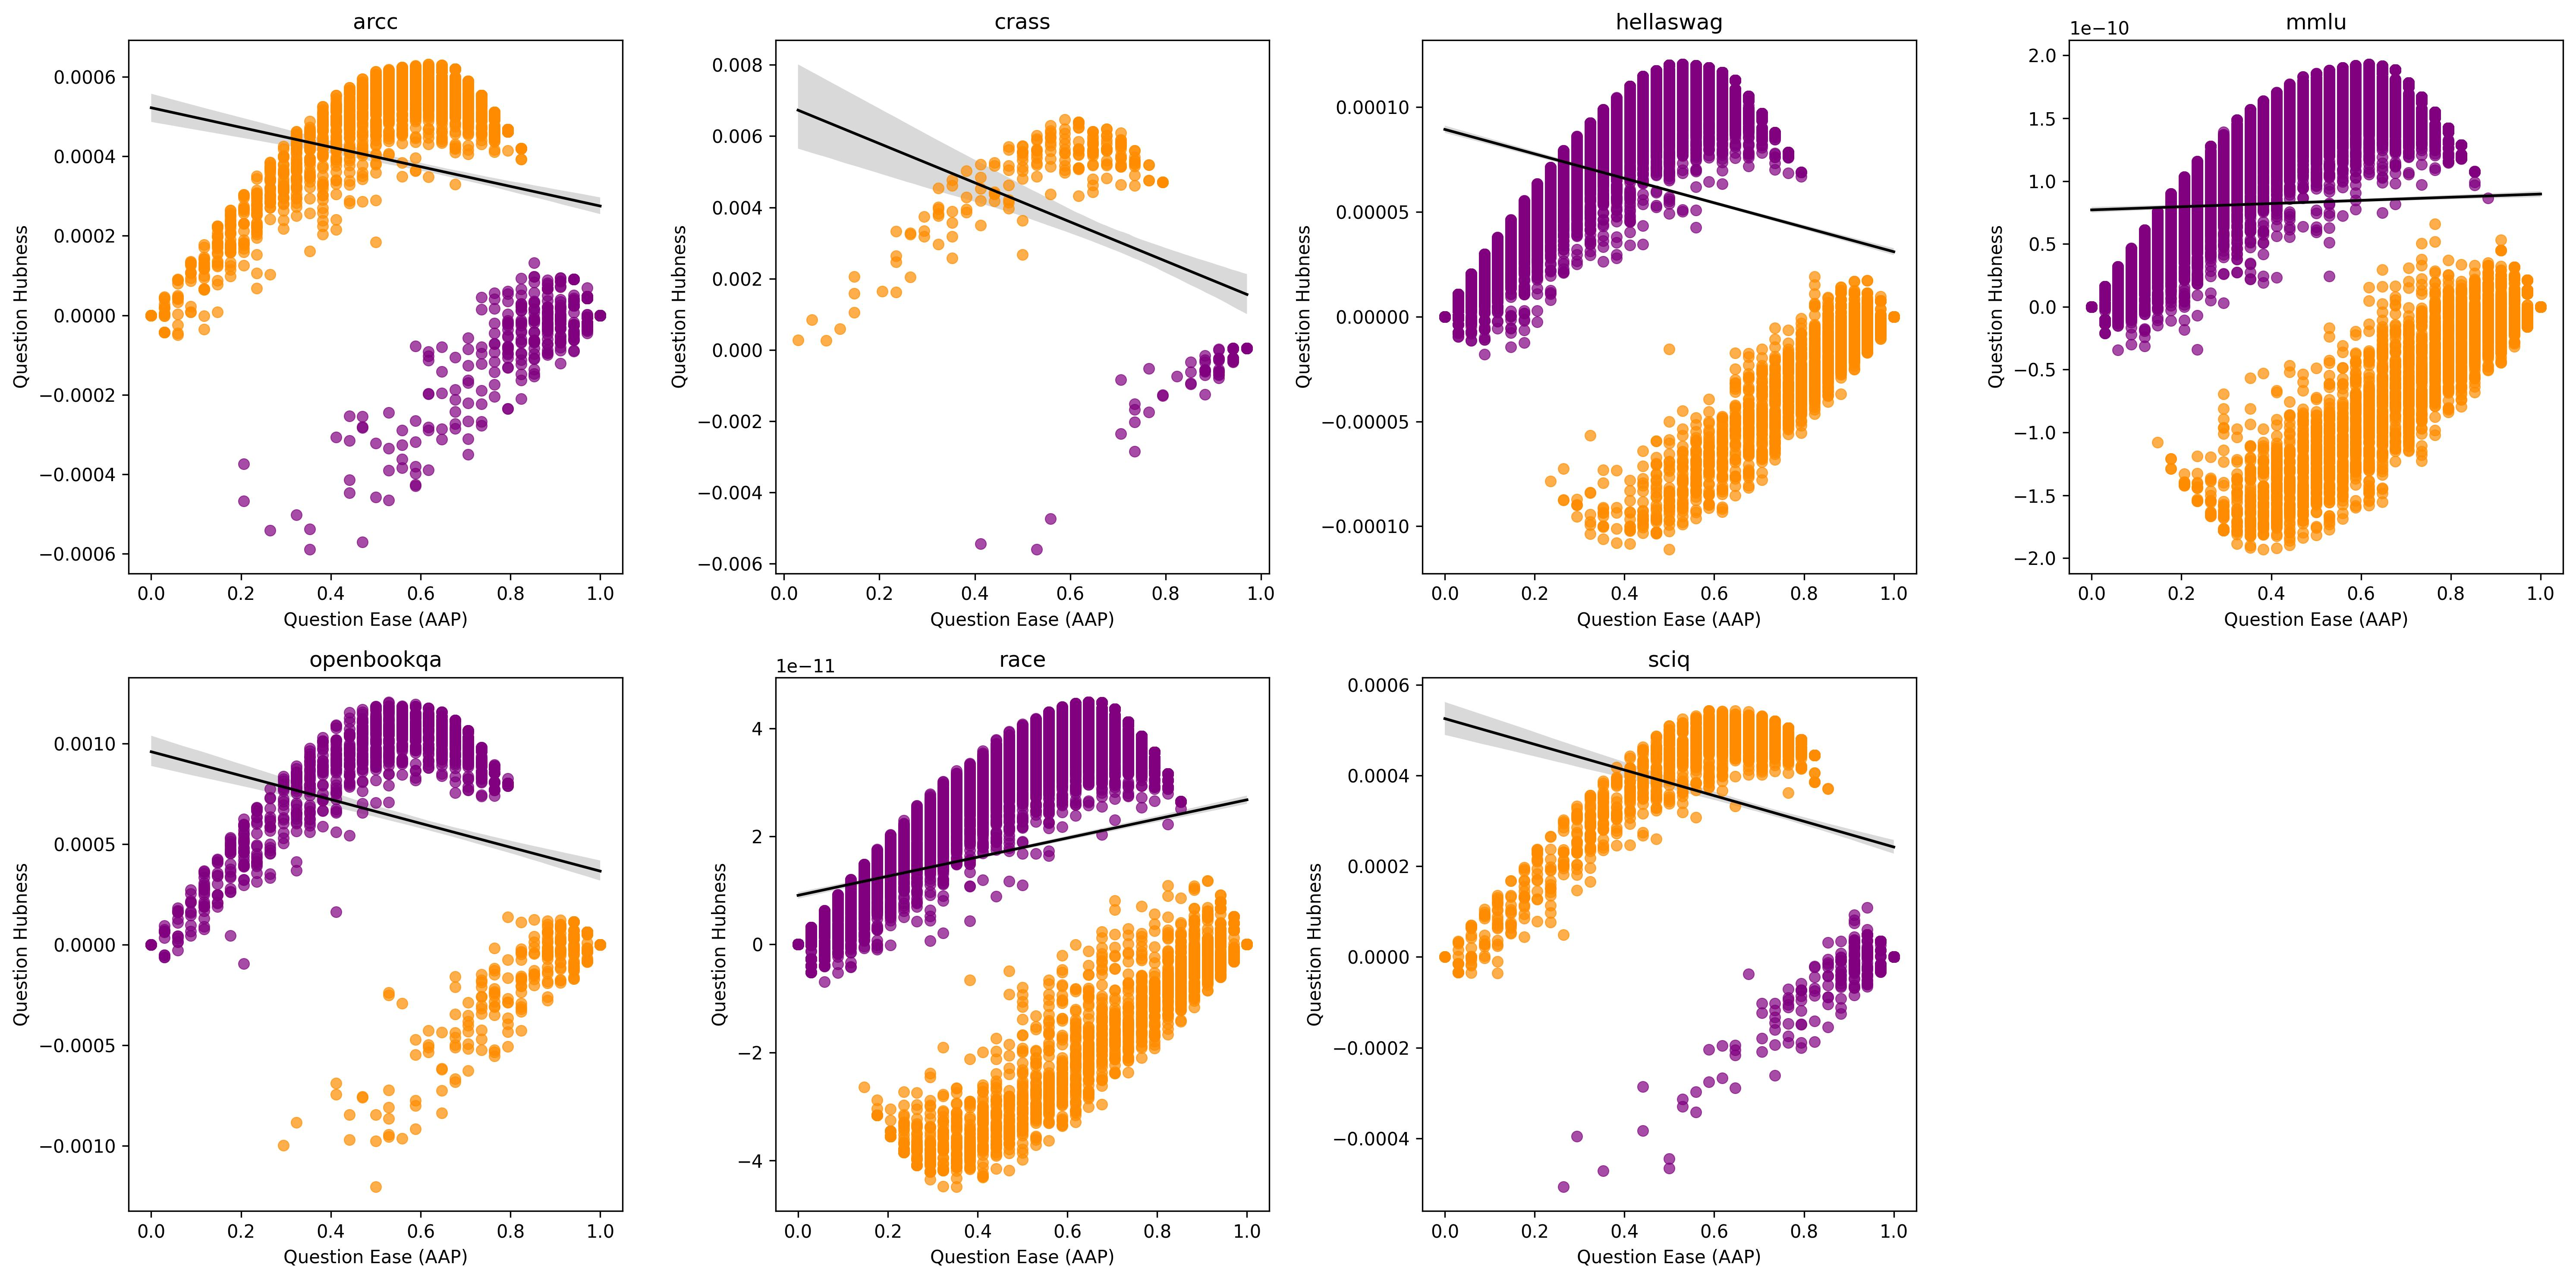
\includegraphics[width=0.9\linewidth]{images/plotsLLM/AAP_vs_Hubness_Questions_all_datasets.jpg}
  \caption{Relazione tra i valori di hubness delle domande e la facilità delle domande (misurata da AAP)}
  \label{fig:Q_AAPvsHUB}
\end{figure}

In generale dai grafici in Figura \ref{fig:Q_AAPvsHUB} si osserva una
correlazione negativa in tutti i dataset, quindi si osserva che domande più
facili (AAP elevato) hanno un valore di hubness più basso. In alcuni dataset si
nota la presenza di due "cluster", in cui anche le domande difficili (AAP
basso) hanno un valore di hubness non massimale, quindi non è il valore più
alto possibile osservato e la loro capacità di discriminare l'efficacia dei
modelli non è la migliore possibile.

Secondo l'algoritmo HITS, un buon hub è un'entità che punta a molte buone
autorità. Quindi, una "domanda hub" è una domanda che viene risposta
correttamente da molti "modello authority" cioè, modelli efficaci. Se le
domande più facili (alto AAP) hanno basso valore di hubness, significa che le
domande facili sono meno brave a discriminare tra modelli efficaci e non.
Questo è sensato perchè se una domanda è troppo facile, allora quasi tutti i
modelli rispondono correttamente. Il trend negativo implica che domande più
difficili (basso AAP) tendono ad avere maggiore valore di hubness, cioè sono
migliori nel discriminare l'efficacia di modelli. Questo ha senso perché sono
le domande più sfidanti che separano i sistemi più efficaci da quelli meno.

La hubness di una domanda indica quanto essa sia discriminante nel distinguere
i modelli più performanti da quelli meno capaci. Le domande facili non svolgono
questa funzione, poiché vengono risolte correttamente dalla maggior parte dei
modelli. Al contrario, le domande difficili costituiscono un banco di prova
ideale per identificare i modelli realmente superiori.

\subsection{Authority vs Question ease (AAP)}

\begin{figure}[H]
  \centering
  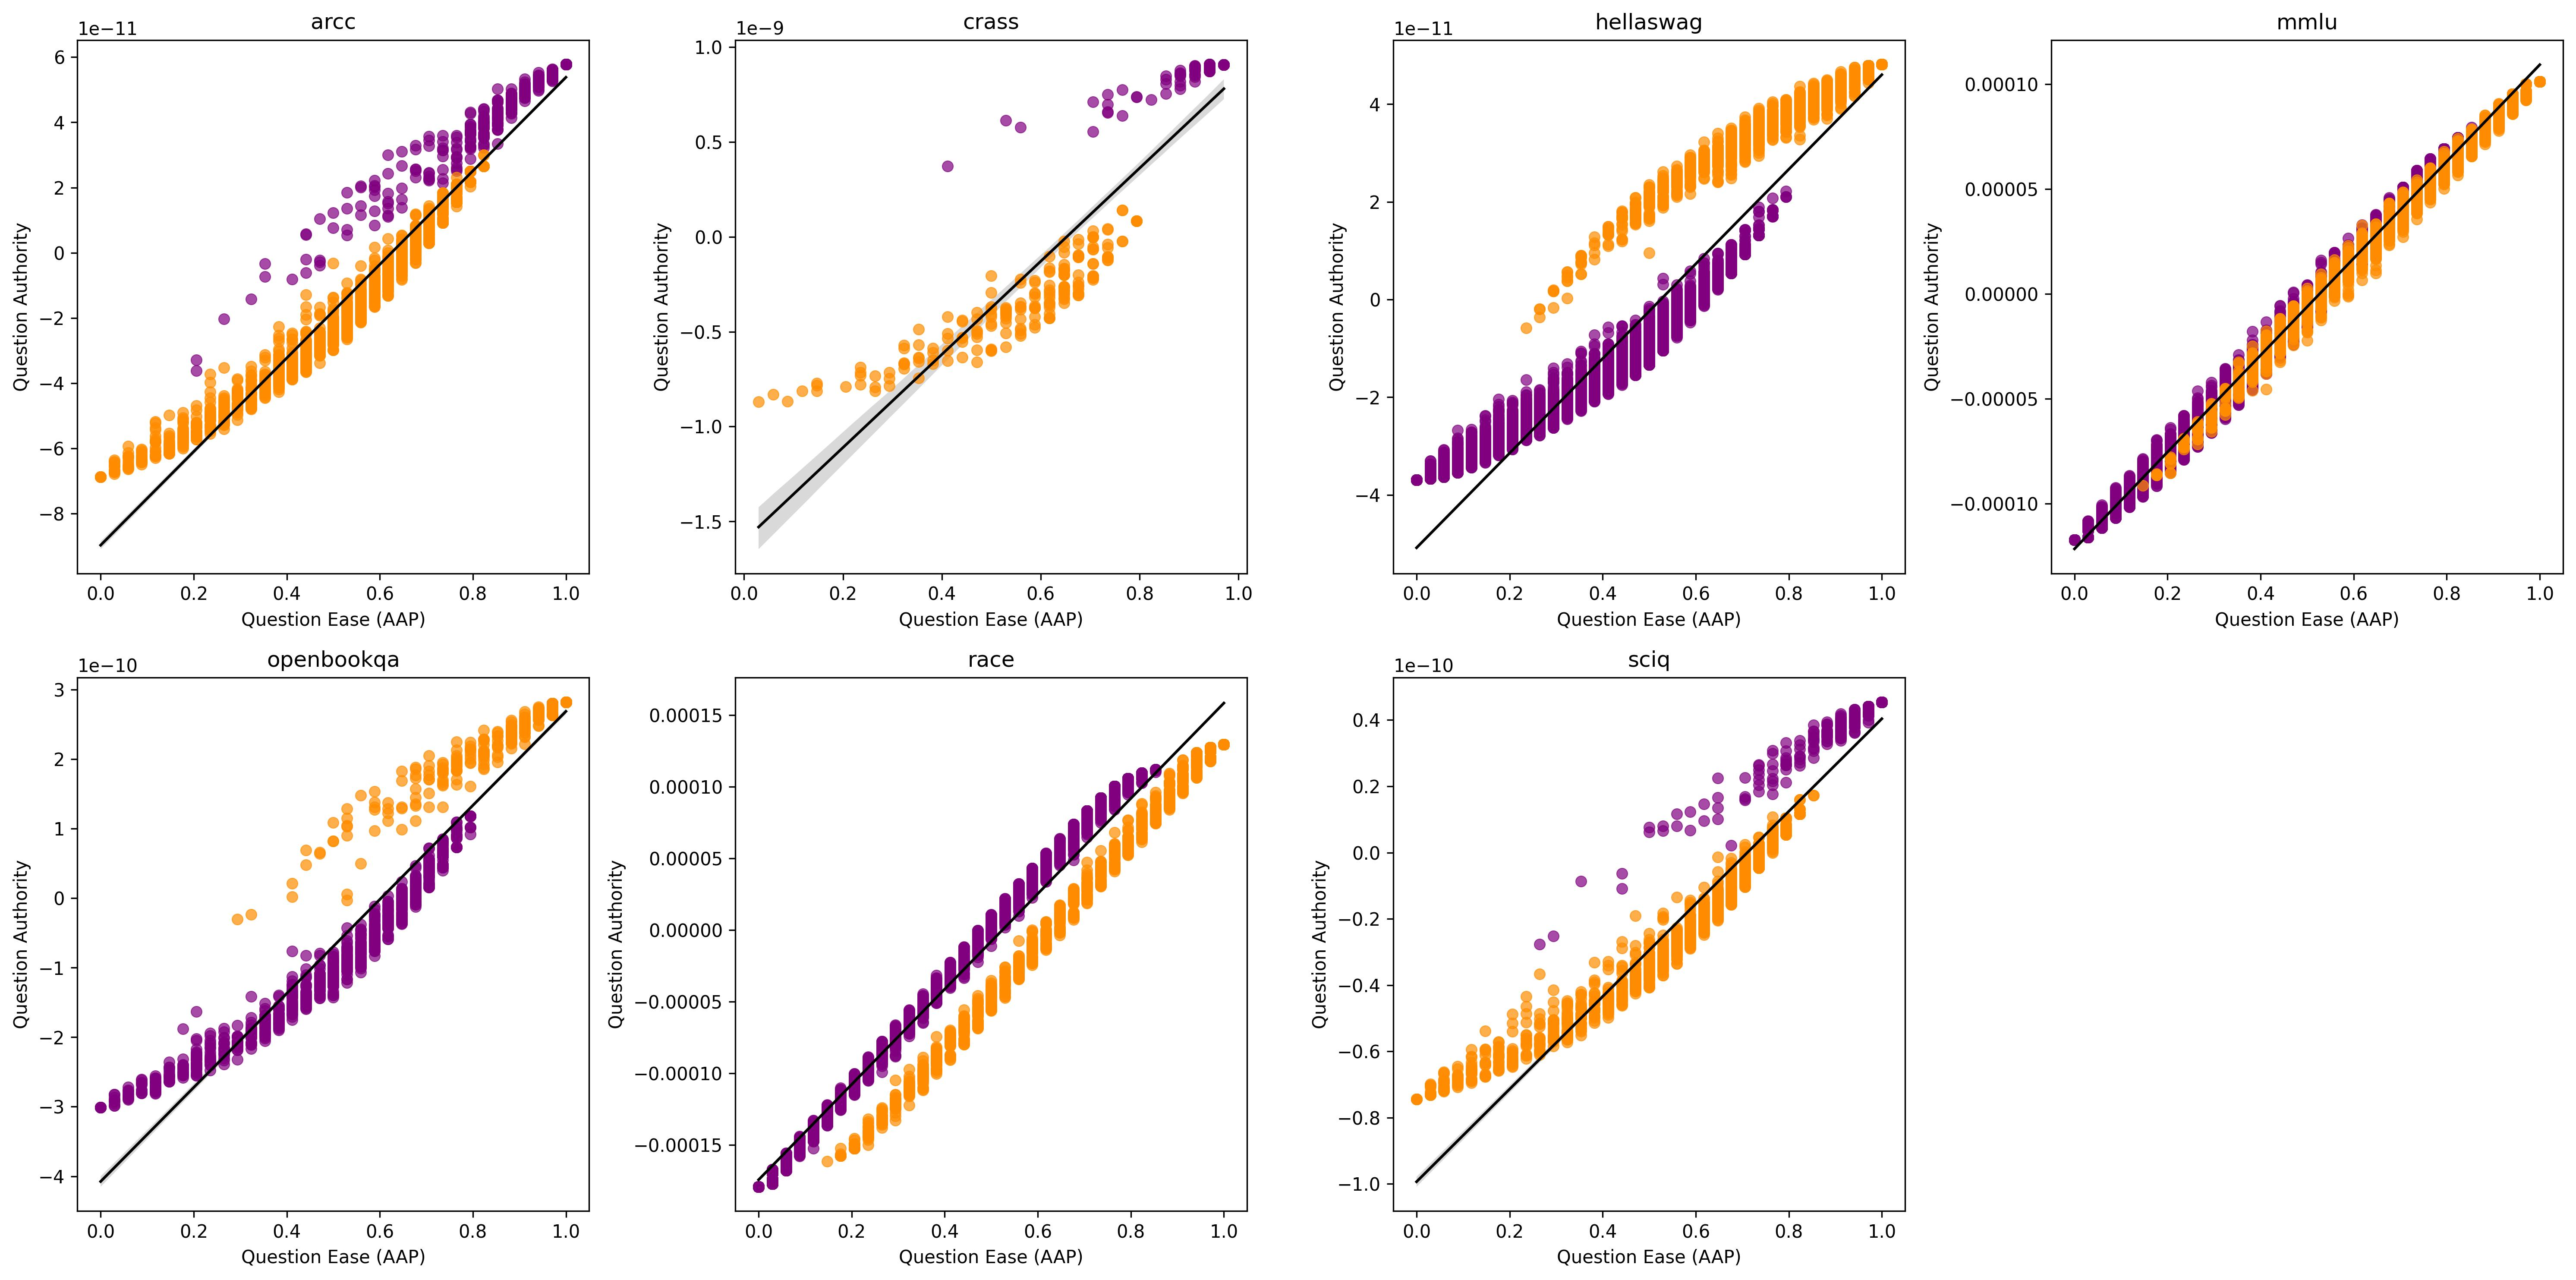
\includegraphics[width=0.9\linewidth]{images/plotsLLM/AAP_vs_Authority_Questions_all_datasets.jpg}
  \caption{Relazione tra i valori di authority delle domande e la facilità delle domande (misurata da AAP)}
  \label{fig:Q_AAPvsAUTH}
\end{figure}

In generale dai grafici in Figura \ref{fig:Q_AAPvsAUTH} si osserva una
correlazione positiva in tutti i dataset, quindi si osserva che domande più
autorevoli (authority alto) hanno un valore di authority più alto.

Secondo l'algoritmo HITS, un'authority è un'entità che è puntata da molti buoni
hub. Quindi, una "domanda authority" (domande facili) è una domanda che è
risposta correttamente da molti "modelli hub", cioè modelli efficaci.

La definizione di "capacità di una domanda di identificare i sistemi più
efficaci" sembra in apparente contrasto con il concetto di "facilità". Infatti,
una domanda facile, per definizione, è risolta da molti sistemi, non solo dai
più efficaci. Tuttavia, se una "domanda authority" è considerata facile e i
"modelli hub" sono quelli specializzati in domande facili (non necessariamente
i più efficaci in generale), allora ha senso che le domande facili siano quelle
a cui i "modelli hub" rispondono. Ovvero, più un sistema è hub, più è in grado
di rispondere a domande facili.

Tuttavia, se interpretiamo la definizione "capacità di identificare i sistemi
più efficaci" come "una domanda che, se un sistema la risolve, indica che il
sistema è efficace", allora le domande facili non sono ideali. Questo ruolo
spetterebbe più alle "domande hub" ovvero quelle che permettono di
discriminare.

Un'interpretazione più probabile è che una "domanda authority" sia una domanda
considerata autorevole (reliable) nel contesto. HITS rileva che queste sono le
domande facili, cioè quelle che sono risolte da molti modelli, specialmente i
"modelli hub". Pertanto la definizione di "authority delle domande" potrebbe
essere ridefinita come una misura della facilità intrinseca della domanda. In
questo modo, il punteggio di authority delle domande riflette la loro facilità
(come misurato dalla correlazione con AAP -> AAP basso = domanda difficile
mentre AAP alto = domanda facile), implicando che le domande più facili
presentino un valore di authority più alto.

L’authority di una domanda potrebbe esprimere il grado di consenso tra i
modelli sulla risposta corretta.

\subsection{Definizioni di hubness e authority post analisi dei grafici}

\paragraph{Hubness dei modelli} Indica la tendenza di un sistema a concentrare le proprie performance corrette
sulle domande più facili (quelle identificate come "domande autorità" da HITS),
il che, come osservato in molti dataset, non sempre correla positivamente con
l'efficacia generale (MAP) del sistema, suggerendo che i modelli più efficaci
non sono necessariamente i migliori "hub" per le sole domande facili;
\paragraph{Authority dei modelli} Emerge come una misura robusta dell'efficacia complessiva di un sistema,
mostrando una forte correlazione positiva con il MAP; questo significa che i
modelli identificati da HITS come "autorevoli" sono effettivamente quelli che
dimostrano prestazioni superiori, in particolare nel rispondere correttamente a
domande discriminanti (le "domande hub");
\paragraph{Hubness delle domande} Quantifica la capacità delle domande di discriminare efficacemente tra modelli
di diversa caratura; le domande con alta hubness sono tipicamente quelle più
difficili (basso AAP), la cui corretta risoluzione è più caratteristica dei
modelli altamente performanti (i "modelli authority");
\paragraph{Authority delle domande} Riflette la facilità intrinseca di una domanda, essendo più elevata per quelle
domande (alto AAP) che vengono risolte correttamente da un'ampia gamma di
sistemi, e in particolare da quei modelli che HITS identifica come "modelli
hub" (orientati alle domande facili).

\section{Confronto caso binario originale con le varie conversioni per il valore 0}

L'analisi della relazione tra AAP e hubness per singola domanda ha rivelato la
presenza di cluster ben definiti. Per verificare se tale raggruppamento fosse
una diretta conseguenza della natura binaria della metrica AP, è stato condotto
un esperimento introducendo valori intermedi per attenuare i cluster. Sono
stati quindi creati due nuovi dataset, sostituendo il valore AP di 0 con 0.1
nel primo e con 0.3 nel secondo.

Il confronto ha mostrato che non vi sono cambiamenti drastici. I cluster
rimangono infatti ben evidenti e definiti in tutte e tre le configurazioni. Da
ciò si evince che la presenza di questi cluster non è dovuta ai valori binari
di AP. La spiegazione più probabile è che tali raggruppamenti riflettano una
struttura intrinseca delle domande stesse, legata ad altri fattori.

\section{Applicazione di HITS sui ranking di domande generati da modelli}

\subsection{Hubness vs. Model effectiveness (MAP)}

\begin{figure}[H]
  \centering
  
\includegraphics[width=0.9\linewidth]{images/plotsLLM_ord/MAP_vs_Hubness_LLM_all_datasets.jpg}
  \caption{Relazione tra i valori di hubness dei modelli e l'efficacia dei modelli (misurata da MAP)}
  \label{fig:MORD_MAPvsHUB}
\end{figure}

Nella maggior parte dei dataset analizzati, la relazione tra MAP e hubness
(Figura \ref{fig:MORD_MAPvsHUB}) assume la forma di una parabola con concavità
rivolta verso il basso. Inizialmente, all'aumentare della performance del
modello, si osserva un corrispondente e graduale aumento dell'hubness. Questa
fase crescente suggerisce che un certo livello di hubness sia una naturale
conseguenza di un sistema efficace.

Tuttavia, superato un punto di massimo, la relazione si inverte: un ulteriore
incremento delle prestazioni diventa controproducente rispetto all’hubness, che
tende a diminuire. In altre parole, i modelli più performanti risultano meno
specializzati nella risoluzione delle domande facili.

Immaginando di percorrere la curva da sinistra a destra, si possono individuare
tre tipologie di modelli:

\begin{itemize}
  \item \textbf{Modelli in basso a sinistra}: sono i meno performanti, caratterizzati da bassa bravura (MAP) e bassa specializzazione sulle domande facili (hubness). In pratica, non eccellono né sulle domande semplici né su quelle complesse.
  \item \textbf{Modelli in salita verso il picco}: rappresentano prestazioni intermedie. Il loro miglioramento è avvenuto innanzitutto consolidando la capacità di rispondere correttamente alle domande facili e di media difficoltà. Il modello posto sul picco è il campione assoluto delle basi, un vero e proprio “maestro” sulle domande semplici/medie.
  \item \textbf{Modelli in discesa dal picco verso destra}: sono i modelli d’élite, con la MAP più elevata. Per raggiungere tali prestazioni, hanno dovuto affrontare con successo le domande più difficili, riducendo però la loro focalizzazione relativa sulle domande semplici.
\end{itemize}

Il grafico evidenzia così due strategie: modelli \emph{generalisti} (sul picco,
eccellenti sulle conoscenze comuni) e modelli \emph{fuoriclasse} (a destra,
performanti anche sulle sfide più estreme). Per diventare un fuoriclasse, un
modello deve accettare di sacrificare parte della propria specializzazione
sulle domande semplici.

Un’eccezione a questo andamento si osserva nel dataset \texttt{hellaswag}, per
il quale la relazione tra MAP e hubness appare pressoché lineare e positiva,
probabilmente a causa della diversa natura del dataset stesso.

\subsection{Authority vs Model effectiveness (MAP)}

\begin{figure}[H]
  \centering
  
\includegraphics[width=0.9\linewidth]{images/plotsLLM_ord/MAP_vs_Authority_LLM_all_datasets.jpg}
  \caption{Relazione tra i valori di authority dei modelli e l'efficacia dei modelli (misurata da MAP)}
  \label{fig:MORD_MAPvsAUTH}
\end{figure}

La relazione tra l'efficacia dei sistemi, misurata da MAP, e l'authority dei
sistemi (Figura \ref{fig:MORD_MAPvsAUTH}) mostra una forte correlazione
positiva. Questo implica che, all'interno di un sistema di valutazione
ordinato, i modelli che dimostrano una maggiore efficacia complessiva sono
anche quelli che acquisiscono il ruolo di "autorità" nella rete.

Ogni punto su questa curva rappresenta un modello. In generale, all’aumentare
del “prestigio” (authority) di un modello corrisponde una maggiore bravura
complessiva (MAP). Il “prestigio” viene assegnato quando un modello risolve con
sicurezza una domanda difficile: è quindi naturale che un modello sia
considerato più performante (alta MAP) proprio perché è capace di affrontare
con successo le domande più impegnative (alta authority).

\subsection{Hubness vs Question ease (AAP)}

\begin{figure}[H]
  \centering
  
\includegraphics[width=0.9\linewidth]{images/plotsLLM_ord/AAP_vs_Hubness_Questions_all_datasets.jpg}
  \caption{Relazione tra i valori di hubness delle domande e la facilità delle domande (misurata da AAP)}
  \label{fig:QORD_AAPvsHUB}
\end{figure}

Analizzando la relazione tra la facilità delle domande, misurata da AAP, e la hubness
dei topic (Figura \ref{fig:QORD_AAPvsHUB}), i grafici mostrano una dispersione
notevole di punti. Si osserva una elevata concentrazione di punti nella parte
sinistra del grafico (corrispondente a valori di AAP più bassi, ovvero domande
più difficili), che tende a disperdersi maggiormente man mano che ci si sposta
verso destra (valori di AAP più alti, ovvero topic più facili). Questa assenza
di una chiara correlazione lineare suggerisce che la "hubness" delle un domande
non è direttamente prevedibile dalla sua difficoltà. Potrebbe indicare che per
i topic più difficili la hubness è più contenuta o raggruppata, mentre per i
topic più facili essa è molto più variabile.

Qui ogni punto rappresenta una domanda. L’utilità di una domanda, misurata
tramite la sua hubness, dipende ora da come i modelli rispondono con
confidenza, rendendo la relazione più complessa del semplice assioma “domanda
difficile = domanda utile”.

Una domanda molto difficile (punto a sinistra nel grafico) potrebbe essere
risolta con bassa confidenza anche dai modelli migliori, risultando quindi poco
efficace nel discriminarli. Al contrario, una domanda di difficoltà media (al
centro) su cui i modelli migliori rispondono con grande sicurezza mentre gli
altri falliscono, assume un valore discriminante elevato (alta hubness).

Quando si considera la confidenza, l’utilità di una domanda per valutare i
modelli non dipende più solo dalla sua difficoltà intrinseca, ma anche da
quanto essa risulti “chiara” e “decisa” per i modelli più performanti,
consentendo loro di fornire risposte sicure. Questa complessità spiega la
dispersione dei punti osservata nel grafico.

\subsection{Authority vs Question ease (AAP)}

\begin{figure}[H]
  \centering
  
\includegraphics[width=0.9\linewidth]{images/plotsLLM_ord/AAP_vs_Authority_Questions_all_datasets.jpg}
  \caption{Relazione tra i valori di hubness delle domande e la facilità delle domande (misurata da AAP)}
  \label{fig:QORD_AAPvsAUTH}
\end{figure}

La correlazione tra la facilità delle domande, misurata da AAP, e l'authority
delle domande (Figura \ref{fig:QORD_AAPvsAUTH}) è anch'essa positiva.
L'andamento generale indica che i topic considerati più facili (con AAP più
elevata) tendono a essere riconosciuti come più "autorevoli" all'interno della
rete. Questa implicazione è contro-intuitiva, ma potrebbe significare che i
topic "autorevoli" sono quelli che molti sistemi riescono a gestire con maggior
precisione.

Qui ogni punto rappresenta una domanda. Il “consenso” (Authority) indica che
molti modelli, in particolare quelli abili nelle domande facili, risolvono
quella domanda con sicurezza. La “facilità” (AAP) misura sostanzialmente lo
stesso concetto: una domanda con alto consenso tra i modelli è necessariamente
una domanda facile.

\section{Analisi di correlazione tra caso binario e caso risposte ordinate}

La seguente analisi confronta i due approcci di valutazione: il caso binario,
che considera le risposte solo come corrette o errate, e il caso ordinato, che
tiene conto di un ranking di confidenza. Ogni grafico a dispersione visualizza
la relazione tra una metrica calcolata con l'approccio binario (asse X) e la
stessa metrica calcolata con l'approccio ordinato (asse Y). La linea rossa di
regressione chiarisce la tendenza generale dei dati, dove una pendenza positiva
indica coerenza tra i due metodi, mentre una pendenza negativa segnala un forte
disaccordo. A supporto dell'analisi grafica è stato calcolato l'indice di
correlazione di Spearman ($\rho$), questi valori sono consultabili in Tabella
\ref{tab:corr}.

\subsection{arcc}

\begin{figure}[H]
  \centering
  
\includegraphics[width=1\linewidth]{images/corr/map_aap/arcc.png}
  \caption{Correlazione tra i valori di MAP per il caso binario e il caso ordinato [grafico a sx]. Correlazione tra i valori di AAP per il caso binario e il caso ordinato [grafico a dx]}
  \label{fig:map_aap_arcc}
\end{figure}

I grafici in Figura \ref{fig:map_aap_arcc} confrontano le metriche MAP (grafico
a sinistra) e AAP (grafico a destra) nel caso binario e ordinato, per il
dataset \texttt{arcc}.

La metrica MAP presenta una forte correlazione negativa. Questo suggerisce che
i due approcci premino strategie opposte: il caso binario favorisce modelli che
massimizzano il numero di risposte corrette, mentre il caso ordinato premia
quelli che posizionano la risposta giusta al primo posto.

Analogamente, la metrica AAP, che misura la difficoltà delle domande, mostra
anch'essa una correlazione negativa. Questo indica che i due approcci
definiscono e valutano la "difficoltà" in modi opposti. L'assunzione è che una
domanda considerata "facile" nel caso binario (cioè, con un AAP binario
elevato, risolta correttamente da molti modelli) venga poi classificata come
"difficile" nel caso ordinato (con un AAP ordinato basso).

I due framework di valutazione premiano strategie prestazionali antagoniste. Il
caso binario favorisce modelli che massimizzano la copertura delle risposte
corrette, anche a bassa confidenza. Il caso ordinato favorisce modelli che
massimizzano la precisione e la confidenza sul ranking della risposta corretta.

\begin{figure}[H]
  \centering
  
\includegraphics[width=1\linewidth]{images/corr/hub_auth_m/arcc.png}
  \caption{Correlazione tra i valori di hubness dei modelli per il caso binario e il caso ordinato [grafico a sx]. Correlazione tra i valori di authority dei modelli per il caso binario e il caso ordinato [grafico a dx]}
  \label{fig:hub_auth_m_arcc}
\end{figure}

\begin{figure}[H]
  \centering
  
\includegraphics[width=1\linewidth]{images/corr/hub_auth_d/arcc.png}
  \caption{Correlazione tra i valori di hubness delle domande per il caso binario e il caso ordinato [grafico a sx]. Correlazione tra i valori di authority delle domande per il caso binario e il caso ordinato [grafico a dx]}
  \label{fig:hub_auth_d_arcc}
\end{figure}

I grafici in Figura \ref{fig:hub_auth_m_arcc} confrontano i valori di hubness
(grafico a sinistra) e authority (grafico a destra) per le domande nel caso
binario e ordinato, per il dataset \texttt{arcc}. Mentre in Figura
\ref{fig:hub_auth_d_arcc} vengono confrontati i valori di hubness (grafico a
sinistra) e authority (grafico a destra) per i modelli nel caso binario e
ordinato.

Si osserva un comportamento coerente sia per le domande che per i modelli.
L'hubness, sia delle domande che dei modelli, mostra in entrambi i casi una
correlazione positiva, indicando che è un concetto stabile e la sua definizione
non dipende dal metodo di valutazione.

La hubness si rivela una proprietà topologica intrinseca della rete
domande-modelli. È un invariante strutturale che descrive la relazione
fondamentale tra la complessità delle istanze e la specializzazione dei
sistemi, a prescindere dal paradigma di valutazione.

Al contrario, l'authority, sia delle domande che dei modelli, presenta una
chiara correlazione negativa. L'ipotesi è che i due approcci abbiano
definizioni diverse di "authority":
\begin{itemize}
  \item Per le domande, il caso binario potrebbe definire "autorevole" una domanda
        semplicemente difficile, mentre il caso ordinato premia quelle che discriminano
        meglio i modelli più performanti;
  \item Per i modelli, l'approccio binario potrebbe considerare "autorevole" un modello
        con molte risposte corrette, mentre quello ordinato privilegia i modelli che
        dimostrano maggiore confidenza sulle domande chiave.
\end{itemize}

L'authority emerge come una proprietà comportamentale e dipendente dal
contesto. Essa non misura una caratteristica immutabile, ma riflette il
successo di un sistema nell'adattarsi a uno specifico regime di valutazione.
Questo sottolinea la relatività del concetto di "autorità" in funzione della
metrica di successo adottata.

\subsection{crass}

\begin{figure}[H]
  \centering
  
\includegraphics[width=1\linewidth]{images/corr/map_aap/crass.png}
  \caption{Correlazione tra i valori di MAP per il caso binario e il caso ordinato [grafico a sx]. Correlazione tra i valori di AAP per il caso binario e il caso ordinato [grafico a dx]}
  \label{fig:map_aap_crass}
\end{figure}

I grafici in Figura \ref{fig:map_aap_crass} confrontano le metriche MAP
(grafico a sinistra) e AAP (grafico a destra) nel caso binario e ordinato, per
il dataset \texttt{crass}.

\begin{figure}[H]
  \centering
  
\includegraphics[width=1\linewidth]{images/corr/hub_auth_m/crass.png}
  \caption{Correlazione tra i valori di hubness dei modelli per il caso binario e il caso ordinato [grafico a sx]. Correlazione tra i valori di authority dei modelli per il caso binario e il caso ordinato [grafico a dx]}
  \label{fig:hub_auth_m_crass}
\end{figure}

\begin{figure}[H]
  \centering
  
\includegraphics[width=1\linewidth]{images/corr/hub_auth_d/crass.png}
  \caption{Correlazione tra i valori di hubness delle domande per il caso binario e il caso ordinato [grafico a sx]. Correlazione tra i valori di authority delle domande per il caso binario e il caso ordinato [grafico a dx]}
  \label{fig:hub_auth_d_crass}
\end{figure}

I grafici in Figura \ref{fig:hub_auth_m_crass} confrontano i valori di hubness
(grafico a sinistra) e authority (grafico a destra) per le domande nel caso
binario e ordinato, per il dataset \texttt{crass}. Mentre in Figura
\ref{fig:hub_auth_d_crass} vengono confrontati i valori di hubness (grafico a
sinistra) e authority (grafico a destra) per i modelli nel caso binario e
ordinato.

\subsection{hellaswag}

\begin{figure}[H]
  \centering
  
\includegraphics[width=1\linewidth]{images/corr/map_aap/hellaswag.png}
  \caption{Correlazione tra i valori di MAP per il caso binario e il caso ordinato [grafico a sx]. Correlazione tra i valori di AAP per il caso binario e il caso ordinato [grafico a dx]}
  \label{fig:map_aap_hella}
\end{figure}

I grafici in Figura \ref{fig:map_aap_hella} confrontano le metriche MAP
(grafico a sinistra) e AAP (grafico a destra) nel caso binario e ordinato, per
il dataset \texttt{hellaswag}.

\begin{figure}[H]
  \centering
  
\includegraphics[width=1\linewidth]{images/corr/hub_auth_m/hellaswag.png}
  \caption{Correlazione tra i valori di hubness dei modelli per il caso binario e il caso ordinato [grafico a sx]. Correlazione tra i valori di authority dei modelli per il caso binario e il caso ordinato [grafico a dx]}
  \label{fig:hub_auth_m_hella}
\end{figure}

\begin{figure}[H]
  \centering
  
\includegraphics[width=1\linewidth]{images/corr/hub_auth_d/hellaswag.png}
  \caption{Correlazione tra i valori di hubness delle domande per il caso binario e il caso ordinato [grafico a sx]. Correlazione tra i valori di authority delle domande per il caso binario e il caso ordinato [grafico a dx]}
  \label{fig:hub_auth_d_hella}
\end{figure}

I grafici in Figura \ref{fig:hub_auth_m_hella} confrontano i valori di hubness
(grafico a sinistra) e authority (grafico a destra) per le domande nel caso
binario e ordinato, per il dataset \texttt{hellaswag}. Mentre in Figura
\ref{fig:hub_auth_d_hella} vengono confrontati i valori di hubness (grafico a
sinistra) e authority (grafico a destra) per i modelli nel caso binario e
ordinato.

\subsection{mmlu}

\begin{figure}[H]
  \centering
  
\includegraphics[width=1\linewidth]{images/corr/map_aap/mmlu.png}
  \caption{Correlazione tra i valori di MAP per il caso binario e il caso ordinato [grafico a sx]. Correlazione tra i valori di AAP per il caso binario e il caso ordinato [grafico a dx]}
  \label{fig:map_aap_mmlu}
\end{figure}

I grafici in Figura \ref{fig:map_aap_mmlu} confrontano le metriche MAP (grafico
a sinistra) e AAP (grafico a destra) nel caso binario e ordinato, per il
dataset \texttt{mmlu}.

\begin{figure}[H]
  \centering
  
\includegraphics[width=1\linewidth]{images/corr/hub_auth_m/mmlu.png}
  \caption{Correlazione tra i valori di hubness dei modelli per il caso binario e il caso ordinato [grafico a sx]. Correlazione tra i valori di authority dei modelli per il caso binario e il caso ordinato [grafico a dx]}
  \label{fig:hub_auth_m_mmlu}
\end{figure}

\begin{figure}[H]
  \centering
  
\includegraphics[width=1\linewidth]{images/corr/hub_auth_d/mmlu.png}
  \caption{Correlazione tra i valori di hubness delle domande per il caso binario e il caso ordinato [grafico a sx]. Correlazione tra i valori di authority delle domande per il caso binario e il caso ordinato [grafico a dx]}
  \label{fig:hub_auth_d_mmlu}
\end{figure}

I grafici in Figura \ref{fig:hub_auth_m_mmlu} confrontano i valori di hubness
(grafico a sinistra) e authority (grafico a destra) per le domande nel caso
binario e ordinato, per il dataset \texttt{mmlu}. Mentre in Figura
\ref{fig:hub_auth_d_mmlu} vengono confrontati i valori di hubness (grafico a
sinistra) e authority (grafico a destra) per i modelli nel caso binario e
ordinato.

\subsection{openbookqa}

\begin{figure}[H]
  \centering
  
\includegraphics[width=1\linewidth]{images/corr/map_aap/openbookqa.png}
  \caption{Correlazione tra i valori di MAP per il caso binario e il caso ordinato [grafico a sx]. Correlazione tra i valori di AAP per il caso binario e il caso ordinato [grafico a dx]}
  \label{fig:map_aap_op}
\end{figure}

I grafici in Figura \ref{fig:map_aap_op} confrontano le metriche MAP (grafico a
sinistra) e AAP (grafico a destra) nel caso binario e ordinato, per il dataset
\texttt{openbookqa}.

\begin{figure}[H]
  \centering
  
\includegraphics[width=1\linewidth]{images/corr/hub_auth_m/openbookqa.png}
  \caption{Correlazione tra i valori di hubness dei modelli per il caso binario e il caso ordinato [grafico a sx]. Correlazione tra i valori di authority dei modelli per il caso binario e il caso ordinato [grafico a dx]}
  \label{fig:hub_auth_m_op}
\end{figure}

\begin{figure}[H]
  \centering
  
\includegraphics[width=1\linewidth]{images/corr/hub_auth_d/openbookqa.png}
  \caption{Correlazione tra i valori di hubness delle domande per il caso binario e il caso ordinato [grafico a sx]. Correlazione tra i valori di authority delle domande per il caso binario e il caso ordinato [grafico a dx]}
  \label{fig:hub_auth_d_op}
\end{figure}

I grafici in Figura \ref{fig:hub_auth_m_op} confrontano i valori di hubness
(grafico a sinistra) e authority (grafico a destra) per le domande nel caso
binario e ordinato, per il dataset \texttt{openbookqa}. Mentre in Figura
\ref{fig:hub_auth_d_op} vengono confrontati i valori di hubness (grafico a
sinistra) e authority (grafico a destra) per i modelli nel caso binario e
ordinato.

\subsection{race}

\begin{figure}[H]
  \centering
  
\includegraphics[width=1\linewidth]{images/corr/map_aap/race.png}
  \caption{Correlazione tra i valori di MAP per il caso binario e il caso ordinato [grafico a sx]. Correlazione tra i valori di AAP per il caso binario e il caso ordinato [grafico a dx]}
  \label{fig:map_aap_race}
\end{figure}

I grafici in Figura \ref{fig:map_aap_race} confrontano le metriche MAP (grafico
a sinistra) e AAP (grafico a destra) nel caso binario e ordinato, per il
dataset \texttt{race}.

\begin{figure}[H]
  \centering
  
\includegraphics[width=1\linewidth]{images/corr/hub_auth_m/race.png}
  \caption{Correlazione tra i valori di hubness dei modelli per il caso binario e il caso ordinato [grafico a sx]. Correlazione tra i valori di authority dei modelli per il caso binario e il caso ordinato [grafico a dx]}
  \label{fig:hub_auth_m_race}
\end{figure}

\begin{figure}[H]
  \centering
  
\includegraphics[width=1\linewidth]{images/corr/hub_auth_d/race.png}
  \caption{Correlazione tra i valori di hubness delle domande per il caso binario e il caso ordinato [grafico a sx]. Correlazione tra i valori di authority delle domande per il caso binario e il caso ordinato [grafico a dx]}
  \label{fig:hub_auth_d_race}
\end{figure}

I grafici in Figura \ref{fig:hub_auth_m_race} confrontano i valori di hubness
(grafico a sinistra) e authority (grafico a destra) per le domande nel caso
binario e ordinato, per il dataset \texttt{race}. Mentre in Figura
\ref{fig:hub_auth_d_race} vengono confrontati i valori di hubness (grafico a
sinistra) e authority (grafico a destra) per i modelli nel caso binario e
ordinato.

\subsection{sciq}

\begin{figure}[H]
  \centering
  
\includegraphics[width=1\linewidth]{images/corr/map_aap/sciq.png}
  \caption{Correlazione tra i valori di MAP per il caso binario e il caso ordinato [grafico a sx]. Correlazione tra i valori di AAP per il caso binario e il caso ordinato [grafico a dx]}
  \label{fig:map_aap_sciq}
\end{figure}

I grafici in Figura \ref{fig:map_aap_sciq} confrontano le metriche MAP (grafico
a sinistra) e AAP (grafico a destra) nel caso binario e ordinato, per il
dataset \texttt{sciq}.

\begin{figure}[H]
  \centering
  
\includegraphics[width=1\linewidth]{images/corr/hub_auth_m/sciq.png}
  \caption{Correlazione tra i valori di hubness dei modelli per il caso binario e il caso ordinato [grafico a sx]. Correlazione tra i valori di authority dei modelli per il caso binario e il caso ordinato [grafico a dx]}
  \label{fig:hub_auth_m_sciq}
\end{figure}

\begin{figure}[H]
  \centering
  
\includegraphics[width=1\linewidth]{images/corr/hub_auth_d/sciq.png}
  \caption{Correlazione tra i valori di hubness delle domande per il caso binario e il caso ordinato [grafico a sx]. Correlazione tra i valori di authority delle domande per il caso binario e il caso ordinato [grafico a dx]}
  \label{fig:hub_auth_d_sciq}
\end{figure}

I grafici in Figura \ref{fig:hub_auth_m_sciq} confrontano i valori di hubness
(grafico a sinistra) e authority (grafico a destra) per le domande nel caso
binario e ordinato, per il dataset \texttt{sciq}. Mentre in Figura
\ref{fig:hub_auth_d_sciq} vengono confrontati i valori di hubness (grafico a
sinistra) e authority (grafico a destra) per i modelli nel caso binario e
ordinato.

L'analisi comparativa condotta sui sette dataset ha fatto emergere un pattern
sistematico e coerente riguardo la stabilità delle metriche.

Le metriche di performance MAP e AAP, così come le metriche di authority (sia
per le domande che per i modelli), hanno evidenziato una correlazione negativa
in tutti i dataset analizzati. Questa tendenza, chiaramente visibile nei
grafici e confermata da coefficienti di Spearman costantemente negativi, le
qualifica come metriche sensibili al contesto.

In netto contrasto, le metriche di hubness, sia per le domande che per i
modelli, hanno mostrato una correlazione positiva. Anche qui, l'analisi visiva
è stata supportata dai coefficienti di Spearman positivi. Questo suggerisce che
il ruolo di "hub" all'interno della rete è una proprietà strutturale meno
influenzata dalla strategia di valutazione scelta.

\begin{table}[H]
  \centering
  \caption{Tabella riassuntiva degli indici di correlazione di Spearman (\(\rho\)) tra caso binario e ordinato per tutti i dataset analizzati.\vspace{0.3cm}}
  \label{tab:corr}
  \begin{tabular}{l S[table-format=-1.4]
      S[table-format=-1.4]
      S[table-format=-1.4]
      S[table-format=1.4]
      S[table-format=-1.4]
      S[table-format=1.4]}
    \toprule
                     & \multicolumn{2}{c}{\textbf{Metriche Performance}} & \multicolumn{2}{c}{\textbf{Proprietà (Modelli)}} & \multicolumn{2}{c}{\textbf{Proprietà (Domande)}}                                                                  \\
    \cmidrule(lr){2-3} \cmidrule(lr){4-5} \cmidrule(lr){6-7}
    \textbf{Dataset} & {\textbf{MAP}}                                    & {\textbf{AAP}}                                   & {\textbf{authority}}                             & {\textbf{hubness}} & {\textbf{authority}} & {\textbf{hubness}} \\
    \midrule
    arcc             & -0.9398                                           & -0.7708                                          & -0.9348                                          & 0.5115             & -0.7176              & 0.6730             \\
    crass            & -0.8881                                           & -0.6146                                          & -0.8520                                          & 0.2263             & -0.7726              & 0.6683             \\
    hellaswag        & -0.9173                                           & -0.8260                                          & -0.9066                                          & 0.8510             & -0.7964              & 0.6604             \\
    mmlu             & -0.9514                                           & -0.8200                                          & -0.9124                                          & 0.6715             & -0.8114              & 0.7422             \\
    openbookqa       & -0.9250                                           & -0.7565                                          & -0.8935                                          & 0.5142             & -0.7328              & 0.7187             \\
    race             & -0.9582                                           & -0.6129                                          & -0.9111                                          & 0.3567             & -0.6056              & 0.5803             \\
    sciq             & -0.9277                                           & -0.7813                                          & -0.9174                                          & 0.5374             & -0.7907              & 0.5840             \\
    \bottomrule
  \end{tabular}
\end{table}

\section{Applicazione di HITS ai dati di TREC con AP discretizzata
 }

L'analisi del dataset TREC si focalizza sull'impatto di diverse strategie di
binarizzazione e discretizzazione applicate ai valori originali e continui di
AP presenti nel dataset. Per la binarizzazione, sono state utilizzate come
soglie la mediana e il terzo quartile, mentre per la discretizzazione sono
stati utilizzati i quattro quartili, suddividendo i valori in quattro fasce
distinte.

\begin{figure}[H]
  \centering
  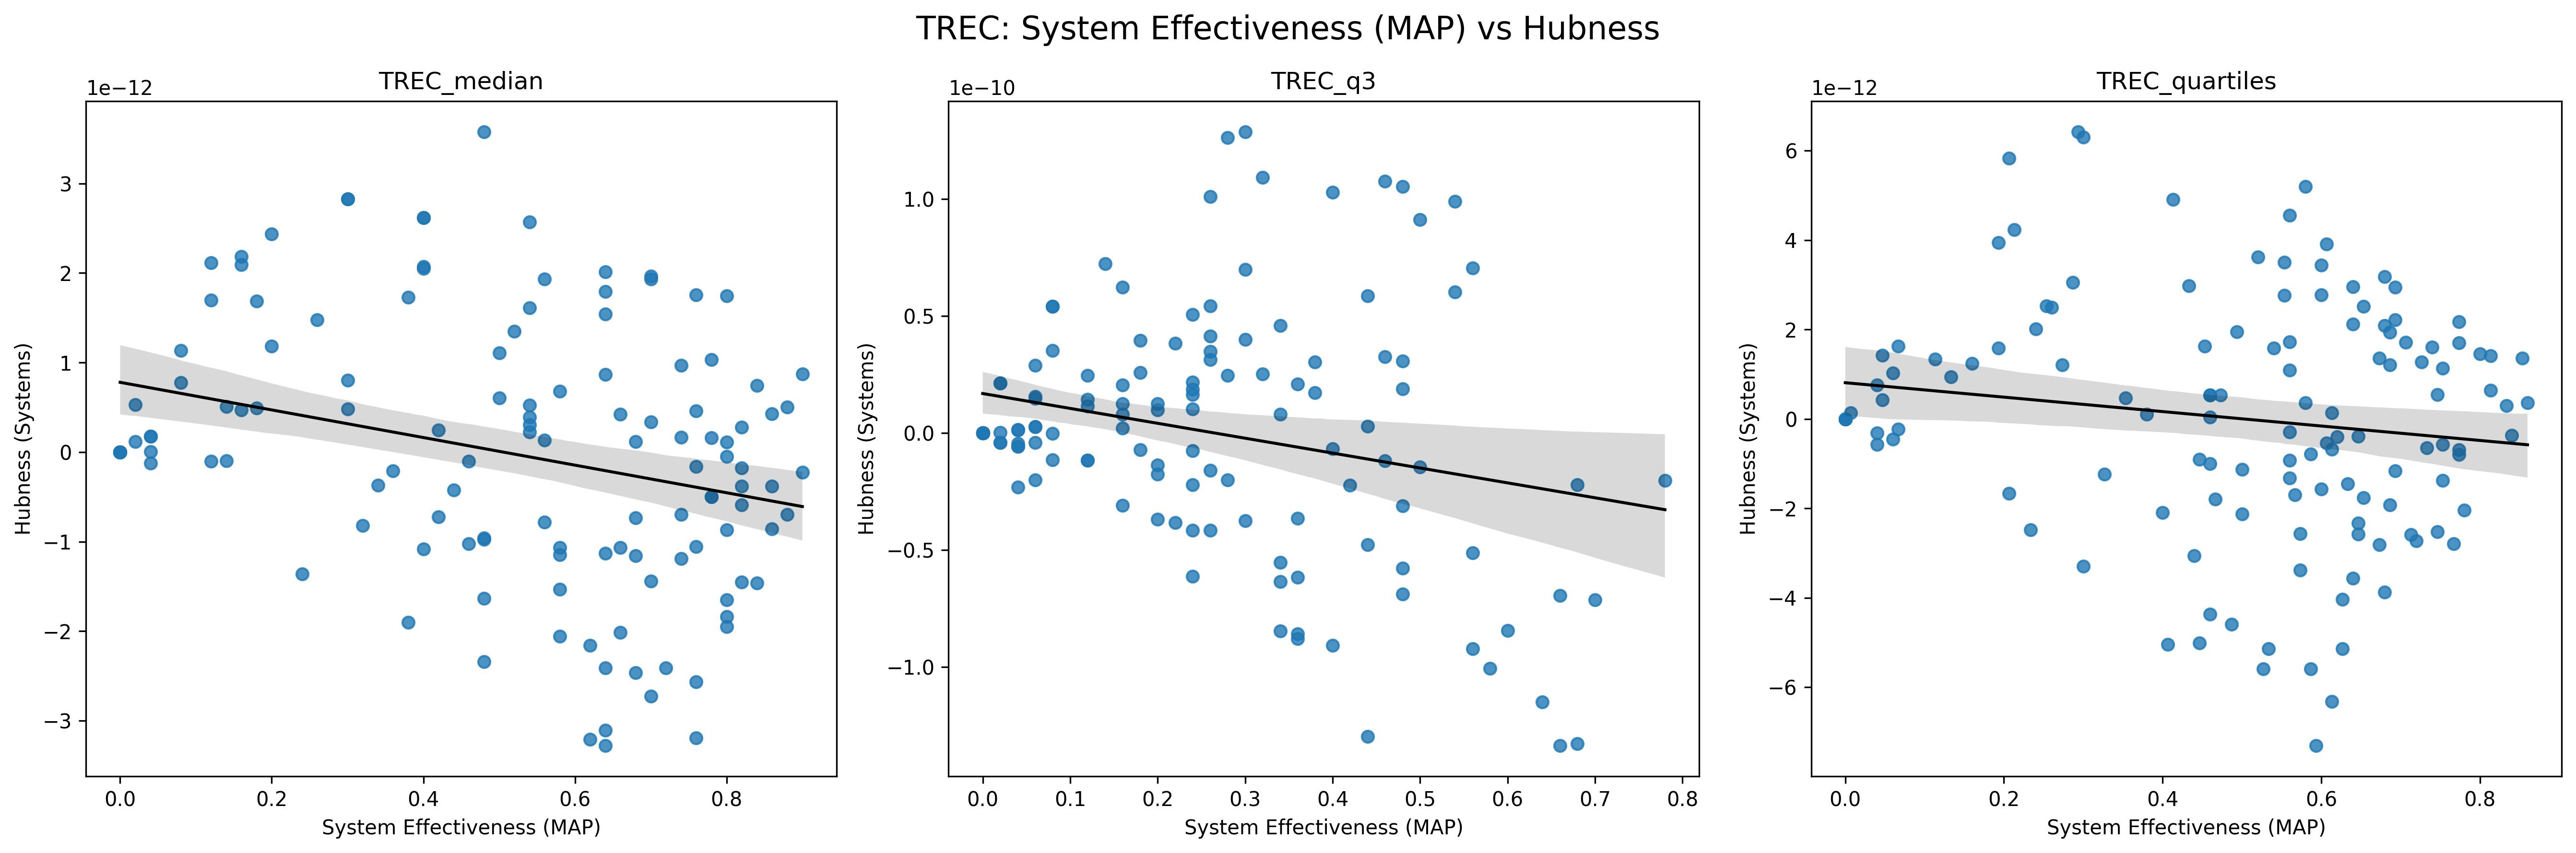
\includegraphics[width=0.9\linewidth]{images/TREC/TREC_MAP_vs_Hubness_Systems_all_datasets.jpg}
  \caption{Relazione tra i valori di hubness dei sistemi e l'efficacia dei sistemi (misurata da MAP)}
  \label{fig:TREC_MAPvsHUB}
\end{figure}

In tutti e tre i grafici presenti in Figura \ref{fig:fig:TREC_AAPvsHUB} si vede
una nuvola sparsa di punti, senza una direzione chiara. Questo ci indica che
nel contesto di TREC, la "specializzazione sul facile" (hubness) di un sistema
e la sua bravura generale (MAP) non sono collegate.

Essere un sistema bravo nel rispondere a topic facili è una caratteristica che
non ci dice nulla sulla qualità complessiva di un sistema. Sono due aspetti
indipendenti. L'hubness, in questo scenario, non è un indicatore utile per
giudicare un sistema.

\begin{figure}[H]
  \centering
  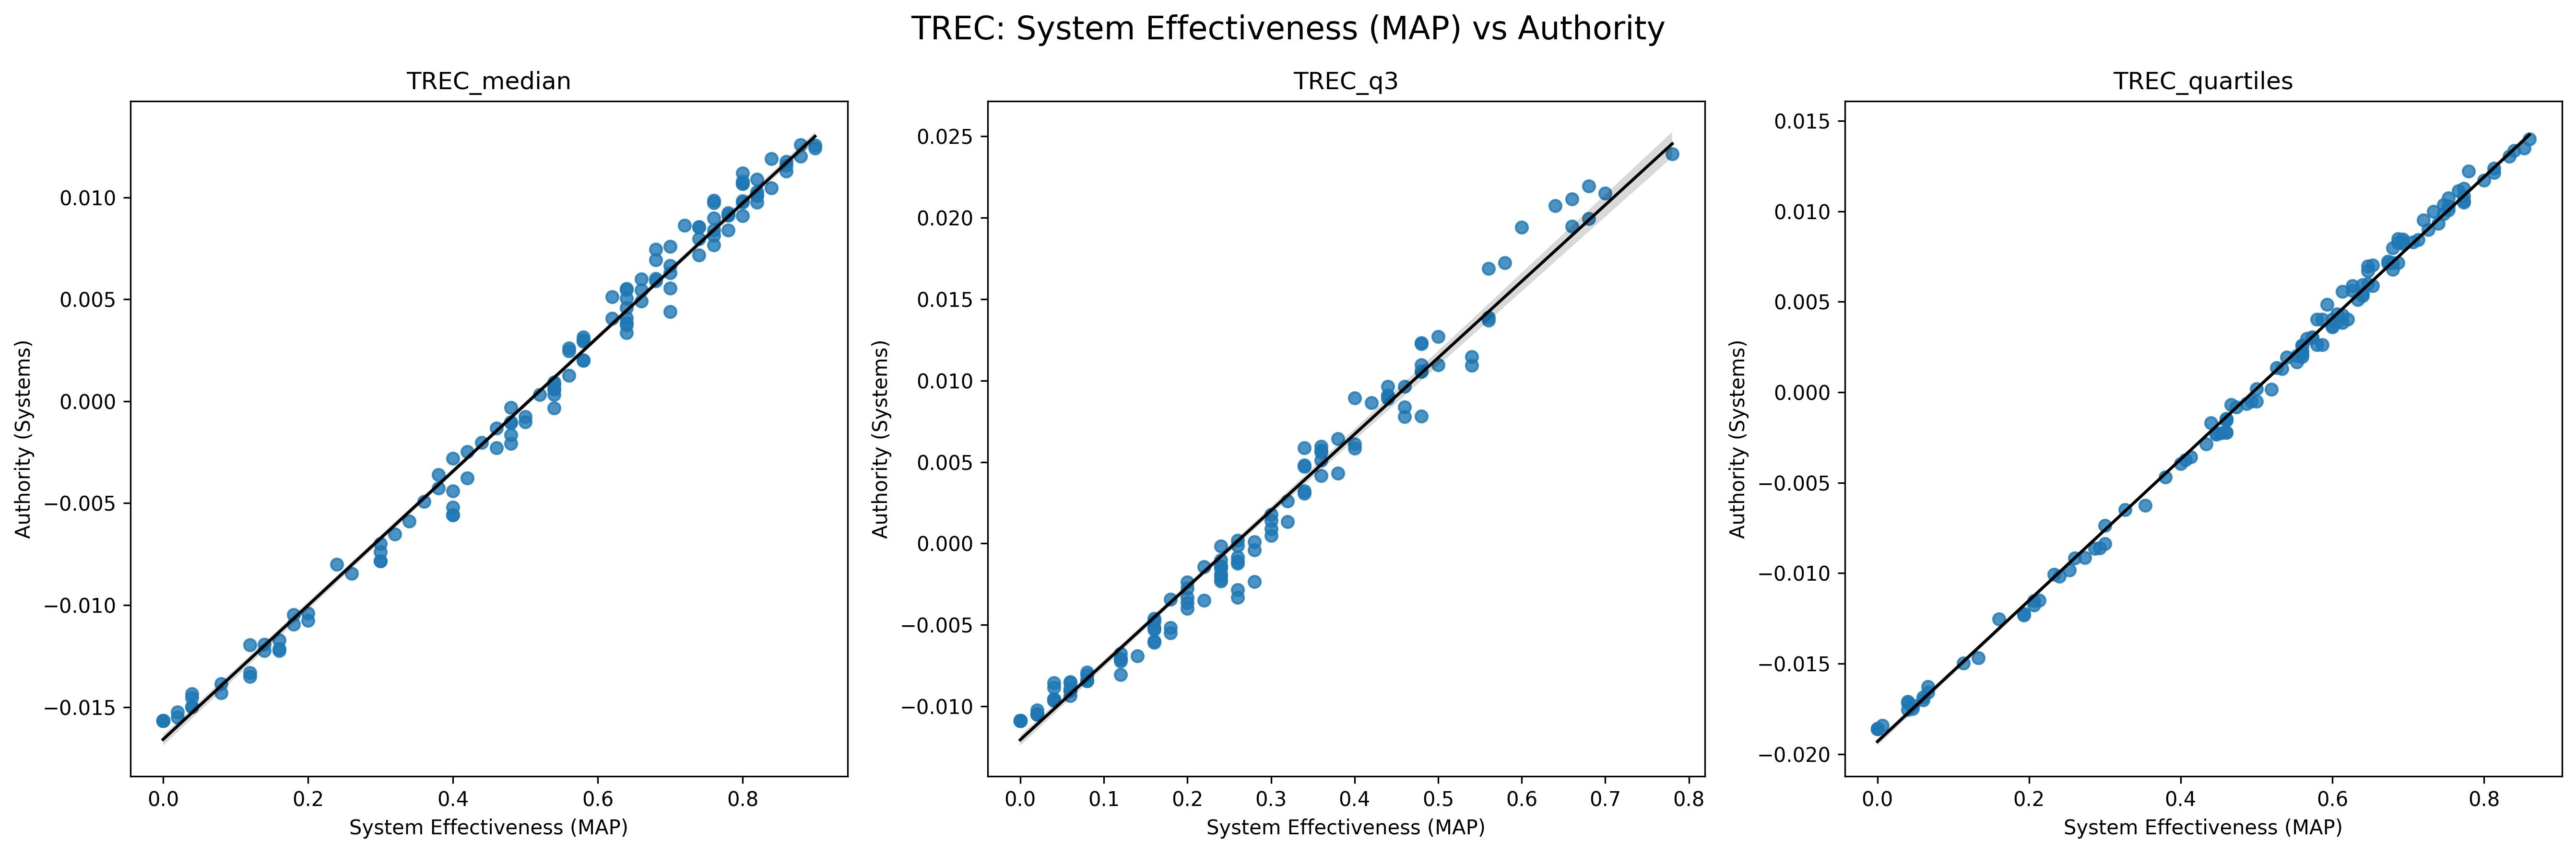
\includegraphics[width=0.9\linewidth]{images/TREC/TREC_MAP_vs_Authority_Systems_all_datasets.jpg}
  \caption{Relazione tra i valori di authority dei sistemi e l'efficacia dei sistemi (misurata da MAP)}
  \label{fig:fig:TREC_MAPvsAUTH}
\end{figure}

Al contrario, dal confronto in Figura \ref{fig:fig:TREC_AAPvsAUTH} tra
authority e l'efficacia del sistema (misurata da MAP) si nota un correlazione
positiva molto forte. Questo significa che il valore di authority di un sistema
e la sua bravura generale sono praticamente la stessa cosa. Se un sistema ha un
alto prestigio, deve essere un sistema bravo, e viceversa.

\begin{figure}[H]
  \centering
  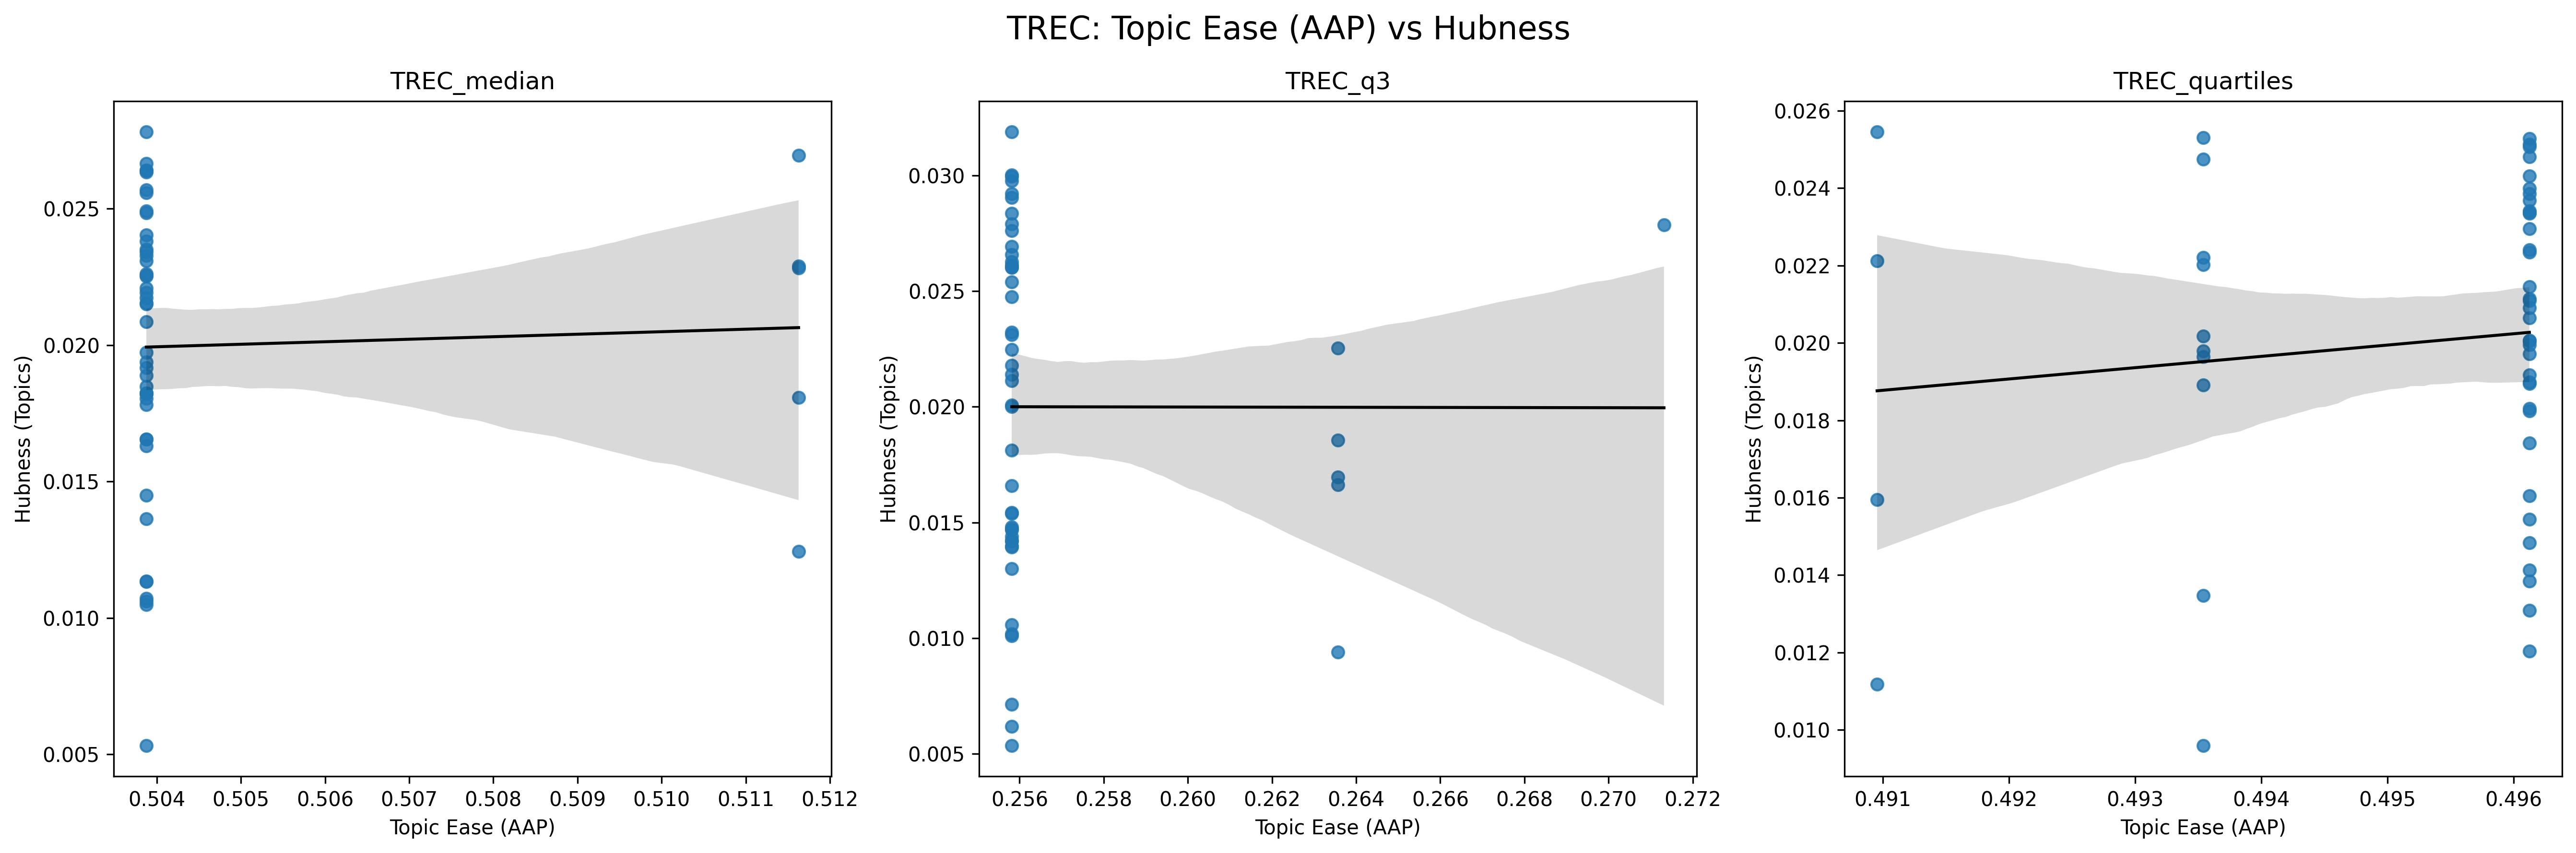
\includegraphics[width=0.9\linewidth]{images/TREC/TREC_AAP_vs_Hubness_Topics_all_datasets.jpg}
  \caption{Relazione tra i valori di hubness dei topic e  la facilità dei topic (misurata da AAP)}
  \label{fig:fig:TREC_AAPvsHUB}
\end{figure}

\begin{figure}[H]
  \centering
  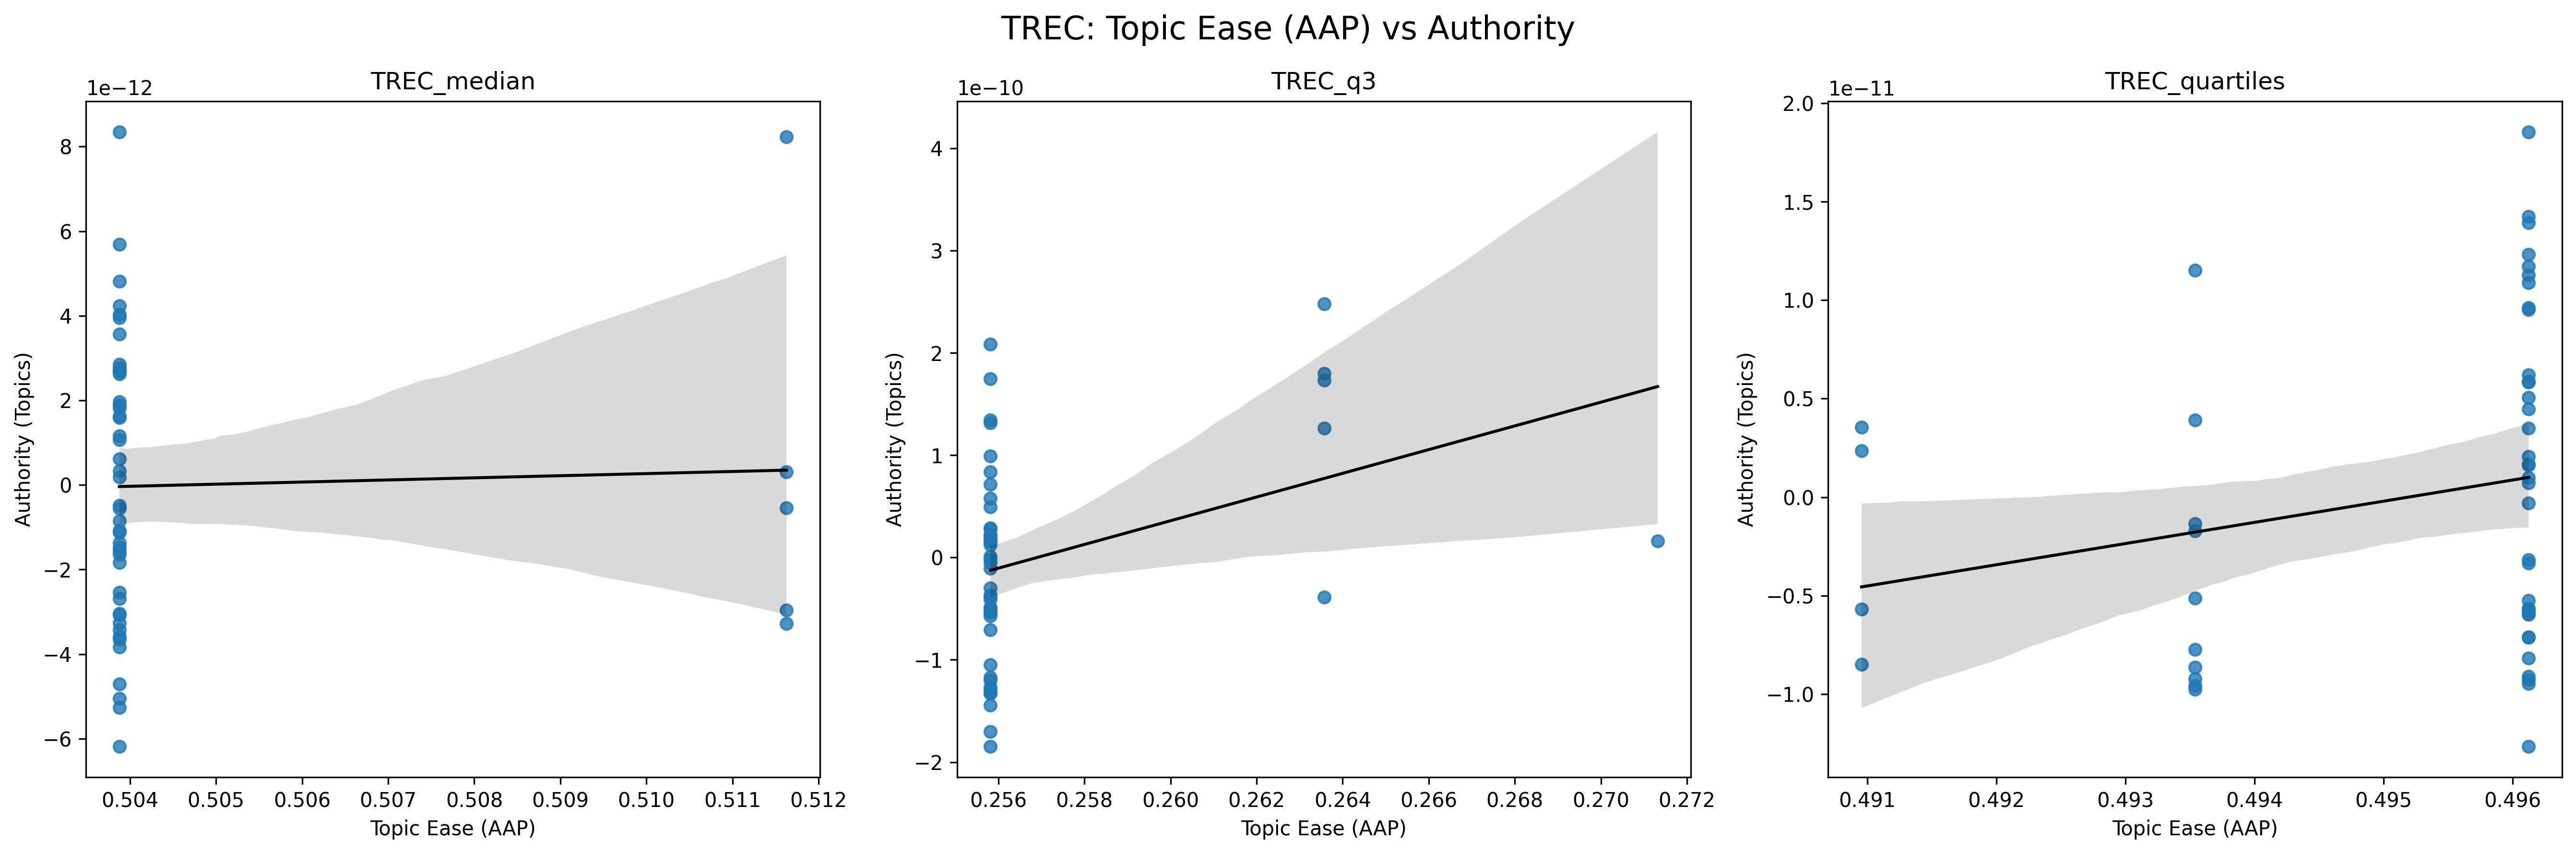
\includegraphics[width=0.9\linewidth]{images/TREC/TREC_AAP_vs_Authority_Topics_all_datasets.jpg}
  \caption{Relazione tra i valori di authority dei topic e  la facilità dei topic (misurata da AAP)}
  \label{fig:fig:TREC_AAPvsAUTH}
\end{figure}

In tutti e tre i casi la relazione tra l'efficacia dei sistemi e la loro
authority è positiva. I grafici mostrano una correlazione forte, con i punti
che si allineano quasi perfettamente lungo la retta di regressione. Questa
stabilità, persistente nonostante la variazione delle soglie di binarizzazione
o l'introduzione di quattro livelli discreti, suggerisce che la performance di
un sistema è un predittore robusto e universale della sua autorità nella rete.

Al contrario, esaminando la relazione tra la difficoltà dei topic e la loro
authority, si nota una correlazione debole e con elevata dispersione. La
presenza di più di due bande, nonostante una binarizzazione a due valori,
indica che i valori di AAP si concentrano in specifici punti lungo l'asse,
indipendentemente dalla soglia applicata. Ciò implica che l'authority di un
topic non è direttamente determinata dalla sua "difficoltà", ma da altri
fattori che ne influenzano il valore.

Analogamente, le relazioni che coinvolgono la hubness si dimostrano deboli in
tutti i contesti. Il legame tra l'efficacia dei sistemi e la loro hubness è
debole e caratterizzata da un'ampia dispersione dei dati. Questo indica che un
sistema altamente efficace non è necessariamente un "hub" nella rete.

Infine, l'analisi della relazione tra la difficoltà dei topic e la loro hubness
rivela una correlazione debole o del tutto assente, con una visualizzazione
simile a quella per l'authority, quindi vale quanto assunto per quel caso. Ciò
implica che l'hubness di un topic non è direttamente determinata dalla sua
"difficoltà", ma da altri fattori che ne influenzano il valore.

\newpage

\end{document}
